% Pro kompilaci po částech (viz projekt.tex), nutno odkomentovat a upravit
%\documentclass[../projekt.tex]{subfiles}
%\begin{document}

\chapter{Úvod}
% Především za poslední 2 roky lze zaznamenat napříč světem vzestup zájmu o umělou inteligenci. Vzniká například mnoho velkých jazykových modelů podporující generativní AI ve formě chatbotů, kteří jsou schopni odpovídat na dotazy na základě dohledatelných dat. Tradiční databázové systémy, jako relační a objektově-relační databáze, jsou efektivní při zpracování strukturovaných dat. Vyhledávání v těchto databázích probíhá nejčastěji konkrétními SQL dotazy. Je to efektivní způsob uchovávání a vyhledávání dat například pro informační systémy. Revoluce AI však přináší práci s daty, která není efektivně nebo vůbec proveditelná těmito databázovými systémy, a proto s ní přichází rozvoj vektorových databází. Ty totiž dokáží pracovat i s nestrukturovanými daty, které jsou reprezentovány pomocí vektorů (matematickou reprezentací n-tice čísel). Svou formou dokáží zachytit význam dat, jako jsou slova nebo celé texty, obrázky a zvuková data. Právě proto patří vektorové databáze k moderním přístupům NLP \cite{vectors_unleashed, co_jsou_vdb}.

Vektorové databáze přináší řešení tam, kde tradiční databázové systémy nestačí. Dokáží pracovat i s nestrukturovanými daty, jako jsou texty, obrázky nebo třeba zvuková data, které reprezentují pomocí vektorů. Svou formou zachycují význam dat, čímž umožňují je sémanticky vyhledávat. Ačkoliv zde techniky a algoritmy sémantického vyhledávání již existují řadu let, řešení ve formě systému správy vektorových databází jsou na vzestupu v posledních 2 letech s revolucí AI. Právě proto patří vektorové databáze k moderním přístupům NLP.

Spojením metod získávání informací na základě významu pomocí vektorových databází a předtrénovaného jazykového modelu lze vytvořit systém, kterému se říká Retrieval-Augmented Generation (RAG), neboli generování rozšířené o získávání informací. Vývoj LLM na vlastních datech je velmi náročný, a proto tento přístup využívá dostupných jazykových modelů. Obohacení dotazování jazykového modelu staví na vlastních zdrojích informací získaných z vektorové databáze, kde je uložen velký objem dat dokumentů. Z~navrácených dat se pak formuje dotaz pro jazykový model společně s dotazem uživatele, který produkuje uživateli odpověď. Tento přístup umožňuje například vyhledávání nad velkým množstvím interních dokumentů firmy, které nebyly a ani nemohly být dostupné při tréninku jazykového modelu. Možnosti využití lze nalézt i v akademickém prostředí při vyhledávání v odborné literatuře. Důležité je zde správné předzpracování dat, jelikož zdroje typicky tvoří velké množství dokumentů různých typů souborů. Vektorové databáze mohou vyhledávat texty, které mají podobný význam jako dotaz, kde vyhledávání na základě klíčových slov nebývá efektivní, pakliže uživatel přesně neví, co hledá. Vyhledané texty pak slouží jako kontext pro odpověď. Data, sloužící jako znalostní báze, je však třeba nejprve vhodně rozkouskovat, přidat k nim metadata a pomocí embedding modelu vytvořit vektorovou reprezentaci, která je uložena do vektorové databáze. 

Cílem kapitoly~\ref{vdb} je tak shrnout fungování vektorových databází pro pochopení následné integrace s jazykovým modelem (systém RAG), které je popsáno v kapitole~\ref{rag}. Výsledkem této práce je pak vytvoření komplexního systému, který nabídne uživatelům získávat informace z velkého množství vlastních dokumentů. Je toho dosaženo kombinací moderních přístupů zpracování přirozeného jazyka, jako jsou zpracování nestrukturovaných dat, embedding modely a vektorové databáze a jejich indexace pro efektivní hybridní vyhledávání k získávání informací. Promptování a generativní schopnosti jazykového modelu nakonec slouží pro navrácení lidsky formulované odpovědi, podložené informacemi z báze znalostí. Architektura tohoto systému se nachází v kapitole~\ref{navrh} a jeho implementační detaily v kapitole~\ref{implementace}. Na závěr, v kapitole~\ref{evaluace}, je experimentálně ověřena úspešnost systému.

\chapter{Vektorové databáze}
\label{vdb}
% co to jsou vektorové databáze
% možná trochu historie - rozdíl oproti klasickým relačním databázím
% definice a jejich význam v moderním kontextu (zpracování nestrukturovaných dat, využití NLP a AI)

\uv{Vektorová databáze je typ databáze, která ukládá data jako vysokorozměrné vektory, což jsou matematické reprezentace rysů nebo atributů.}~\cite{compreh_survey_vdb}. Vektorové databáze jsou relativně moderní technologií, která vznikla především jako řešení na zpracování a vyhledávání nestrukturovaných dat. Již v roce 1998 bylo odhadováno, že více než 85\% dat neexistuje ve strukturované formě, a tedy je nelze uložit do relačních databází~\cite{problem_with_unstructured}. Před zhruba deseti lety začaly s vývojem zpracování přirozeného jazyka a hlubokého učení vznikat trénované modely. Tyto modely dokáží převést nestrukturovaná data do vektorové reprezentace, která zachovává jejich význam a vlastnosti. Aby však existovala možnost s těmito vektory efektivně pracovat, vznikla specializovaná databáze. V důsledku tomu začal během posledních let vývoj tvorby vektorových databází, kde uložení velkého množství vektorů je jen prvním krokem. Síla těchto systémů plyne z efektivního vyhledávání na základě sémantické podobnosti, zatímco relační databáze provádějí vyhledávání skrze sloupce a porovnávání hodnot. To je klíčové pro moderní aplikace, jako jsou doporučovací systémy, chatboti nebo vyhledávače obrázků. V následujících podkapitolách je detailněji popsáno, jak vektorové databáze zpracovávají nestrukturovaná data, jak funguje vektorová reprezentace dat a jak se provádí indexace pro efektivní vyhledávání.

\section{Nestrukturovaná data}
% co jsou unstructured data
% jake prinasi vyzvy a role VDB 
Lidé i stroje produkují velké množství dat, které nesplňují předem daný formát nebo schéma. Taková data jsou pak náročná na vyhledávání a vyžadují předzpracování a analýzu. Nestrukturovaná data nezapadají do relačních databázových systémů, jelikož je nelze reprezentovat hodnotami uloženými do sloupců tabulky jako data strukturovaná. V jejich kontextu spadají do datového typu BLOB (Binary Large Object), přes které nelze snadno vyhledávat. 

Příkladem nestrukturovaných dat jsou~\cite{zilliz_unstructured_data}:
\begin{itemize}
    \item \textbf{Data vytvořená člověkem}: E-maily, textové dokumenty, poznámky, obrázky, audio nebo video nahrávky,
    \item \textbf{Data vytvořená strojem}: Údaje ze senzorů, data počítačového vidění, webová a aplikační data, logy, data z IoT zařízení.
\end{itemize} 

Mezi strukturovanými a nestrukturovanými daty existuje mezikrok, který se nazývá polostrukturovaná data. Vznikají přidáním metadat nebo významových tagů, čímž je dodána nestrukturovaným datům jistá forma organizace nebo hierarchie. Například k obrázkům, které jsou binárním popisem vlastností jednotlivým pixelů, lze přidat údaje o autorovi a datu a místa vzniku, což umožňuje snadnější filtrování a organizaci dat~\cite{semi-structured}.

Nestrukturovaná data jsou nejen ukládána, ale procesem vektorizace je jim přidělena sémantika~\cite{vdbms}. Proto pro efektivní uložení a vyhledávání nestrukturovaných dat hrají klíčovou roli systémy pro správu vektorových databází.
 
\section{Vektorová reprezentace dat}
Vektor je v matematice formálně definován jako prvek vektorového prostoru. Pakliže má tento prostor konečné rozměry, lze hovořit o uspořádané n-tici čísel, kde $n$ udává dimenzi vektoru. S vektory lze provádět operace vektorové aritmetiky, kde nejdůležitější roli pro vektorové databáze hrají podobnostní funkce jako kosinová podobnost, Euklidovská vzdálenost nebo skalární součin~\cite{wolfram_vector}.

V kontextu vektorových databází jsou vektory tvořeny transformací dat na matematickou reprezentaci pomocí modelů strojového učení, které se nazývají embedding modely~\cite{compreh_survey_vdb}. Vektory si tedy lze představit jako soubor čísel, kde každé z nich reprezentuje číselné vyjádření určité vlastnosti dat. Např. na obrázku \ref{fig:vector2D} je zobrazen 2D prostor, pakliže jednotlivým složkám dvourozměrného vektoru přidělíme nějaký rys, můžeme ohodnotit např. slova označující ovoce, kde první hodnota bude sladkost a druhá hodnota kyselost (na škále 1-10) a uložit je do tohoto vektorového prostoru.

\begin{figure}[H]
    \centering
    \includegraphics[width=0.5\linewidth]{placeholder.pdf}
    \caption{Příklad vektorového prostoru o 2 dimenzích. Podobnost vlastností dat lze vypočítat vzájemnou vzdáleností mezi vektory, a tak významově podobná data jsou blízko sebe.}
    \label{fig:vector2D}
\end{figure}

Komplexní data však vyžadují mnohem více popisů atributů, a tak podobně jako nestrukturovaná data, vysocedimenziální vektory nejsou pro lidi čitelné a uchopitelné. Pro práci s vektory není nutné užití specializovaných vektorových databází, avšak jak počet vektorů a jejich dimenze roste, vektorový databázový systém poskytuje efektivní řešení pro uložení a vyhledávání nad těmito komplexními daty~\cite{vdbms}. Počet dimenzí vektorů se snadno pohybuje od stovek po tisíce, s tím že s vývojem poroste na desítky tisíc. Toto číslo se odvíjí od architektury použitého embedding modelu.

\section{Embedding modely}
Proces vektorizace lze označit jako \uv{transformaci dat na vysocedimenzionální vektorovou reprezentaci, která zachycuje smysluplné vztahy a vzorce}~\cite{vdbms}. Cílem embedding modelů je zachytit význam dat v numerické podobě, aby byly použitelné pro výpočetní modely. Výsledné vektory, též nazývané \textit{embeddingy}, umožňují strojům práci s nestrukturovanými daty, jelikož jejich poloha v prostoru odráží vzájemné vztahy s ostatními vektory. Významově podobná vstupní data tak budou blízko sebe. Demonstraci vektorové aritmetiky a vzájemného vztahu mezi daty uloženými ve vektorovém prostoru lze ilustrovat na klasickém příkladu~\cite{illustratedw2c}: Mějme vektorový prostor obsahující vektorové reprezentace slov ze slovníku. Mějme vektorovou reprezentaci slova \textit{král}. Odečteme-li od slova \textit{král} slovo \textit{muž} a následně přičteme slovo \textit{žena}, nejbližší vektor tomuto vypočtenému vektoru bude ten, který reprezentuje slovo \textit{královna}.

\begin{figure}[H]
    \centering
    \includegraphics[width=0.5\linewidth]{placeholder.pdf}
    \caption{}
    \label{fig:vector2D}
\end{figure}

Embedding modely jsou jedním z produktů strojového učení. Obecně vznikají trénováním na rozsáhlých sadách nestrukturovaných dat, např. textových korpusech, obrázcích nebo zvukových souborech. Tato práce se specificky zaměřuje na zpracování textových dokumentů, kde embedding modely patří k významnému nástroji zpracování přirozeného jazyka. 

\subsection{Word Embeddings}
Prvním průlomem ve vývoji embedding modelů byly \textit{word embeddings}, které vektorizují jednotlivá slova. Pro proces konverze se používají nástroje jako Word2vec, který využívá neuronové sítě k naučení asociace slova z velkého textového korpusu. Word2vec byl navržen jako 2 modely~\cite{from_word_to_sense}, kde:
\begin{itemize}
    \item \textbf{CBOW} (Continuous Bag-Of-Words) se zaměřuje na předpovídání aktuálního slova na základě okolního kontextu, zatímco
    \item \textbf{Skip-gram} se na rozdíl od CBOW zaměřuje na předpovídání kontextu pro dané slovo.
\end{itemize} 
Dalším významnou architekturou je GloVe (Global Vectors)~\cite{glove}.

Cíl reprezentovat každé slovo bodem ve vektorovém prostoru má hlavní nedostatek, jelikož ignoruje možnosti slova, které má v různých kontextech různý význam. Problémem word embeddings tak je, že vícevýznamová slova jsou přeložena v každém svém významu ve větě na identickou vektorovou reprezentaci. Zachycení správné sémantiky vícevýznamových slov však hraje klíčovou roli v porozumění jazyku NLP systémů. Může se tak stát, že slova \textit{krysa} a \textit{počítač} budou \uv{blízko sebe}, ačkoliv spolu sémanticky nesouvisí, jelikož se budou obě významově blížit slovu \textit{myš}~\cite{from_word_to_sense}.

\subsection{Kontextové modely}
Moderní kontextové embedding modely, jako jsou BERT nebo GPT, patří mezi velké jazykové modely (LLM). Mimo sumarizaci a prediktivní generování textu dokáží tyto LLM tvořit vektorové reprezentace textu. Umí zachytit dynamiku vícevýznamových slov tak, že pro různé významy slov generují různé vektorové reprezentace. Zohledňují tak kontext konkrétní věty na základě okolních slov.

\subsubsection{GPT (Generative Pre-Trained Transformer)}
Příkladem kontextového modelu je GPT, funguje na architektuře transformerů a byl navržen pro generování textu. Predikuje další slovo ve věte na základě předchozích slov a kontext slova dokáže zachytit tím, že čte větu jednosměrně zleva doprava. Mimo generování textu však dokáže díky porozumění kontextu vytvářet vektorové repezentace textu~\cite{gpt}.

\subsubsection{BERT (Bidirectional Encoder Representations from Transformers)}
BERT je předtrénovaný model (převážně na celé anglické Wikipedii), který používá transformery k zachycení kontextu slova ve větě, kterou navíc čte oběma směry, zleva doprava i zprava doleva. Tím dokáže lépe zachytit kontext daného slova a vytvořit pro něj vektorovou reprezentaci~\cite{bert}.

\subsubsection{S-BERT (Sentence-BERT)}
S-BERT je rozšíření modelu BERT. Oproti předchozím modelům je S-BERT efektivnějším nástrojem pro zpracování textových dokumentů, jelikož optimalizuje tvorbu vektorové reprezentace vět (\textit{sentence embeddings}). Přidává speciální tréninkovou fázi, aby mohl efektivně vytvářet vektory z celých kusů textu~\cite{sbert}. Toho lze využít ve vektorových databázích při uložení textových dokumentů a následném vyhledávání pomocí dotazu vektorizovaném tímto modelem.

\section{Systém správy vektorových databází}
Systém správy vektorových databází je technologie, která práci s vektorovými databázemi seskupuje dohromady. Je to specializovaný typ systému správy databází zaměřující se na efektivní správu vysokorozměrných vektorových dat. Toto nezahrnuje nízkorozměrná vektorová data (jako například 2D souřadnice) s nimiž je práce podstatně jednodušší a nevyžaduje dále uvedené optimalizační techniky. VDBMS (z anglického Vector Database Management System) většinou podporuje vyhledávání na základě podobnosti postřednictvím indexace, které je nevyhnutelné pro rychlé vyhledávání ve vektorovém prostoru~\cite{vdbms}.

Termín vektorová databáze se často používá jako synonymum pro VDBMS. Sama vektorová databáze je však jen soubor dat, zatímco systém správy vektorových databází je celý software. Zajišťuje nejen uložení dat, ale i efektivní navracení relevantních informací a často si ukládá k samotnému vektoru i nějaký identifikátor nebo metadata, která mohou sloužit k filtrování nebo k poskytování personalizovaných doporučení~\cite{vdbms}.

Mezi známé systémy správy vektorových databází patří~\cite{survey_vdb}:
\begin{itemize}
    \item \textbf{Weaviate} – open-source databáze s podporou hybridního vyhledávání, která se zaměřuje na vyhledávání dokumentů v grafovém modelu.
    \item \textbf{Pinecone} – proprietární řešení zaměřené na škálování nabízen jako cloudový systém.
    \item \textbf{Milvus} – systém podporující vícenásobné indexovací metody a distribuci výpočtů.
    \item \textbf{Qdrant} – databáze s důrazem na filtrování podle metadat a API přívětivé rozhraní.
    \item \textbf{Faiss} – knihovna společnosti Meta s algoritmy pro indexaci a vyhledávání s vektory.
    \item \textbf{pgvector} – rozšíření PostgreSQL, které přidává vektor a indexační metody pro vektorové vyhledávání.
\end{itemize}


\section{Indexace a vyhledávání}
\label{index}
Po vektorizaci a uložení dat je nad nimi potřeba vytvořit index. Indexace slouží k organizaci dat pro rychlejší vyhledávání. Vektorové indexy zrychlují proces vyhledávání minimalizací porovnávání vektorů rozdělením vektorového prostoru na datové struktury, které lze snadno procházet. Porovnává se tak pouze malá podmnožina prostoru k nalezení nejbližších sousedů~\cite{survey_vdb}.

Výběr algoritmu k indexaci záleží na požadavcích. Obecně bývá výpočetně náročný, v ideálním případě ho však není třeba při rozšíření datasetu přepočítávat a umožňuje velmi rychlé vyhledávání. Právě proto se bez něho VDBMS neobejdou~\cite{vdbms}.

Dotazování pak předchází vyhledávání. Dotazy jsou podávány systému často v přirozeném jazyce, a proto potřebují být taktéž vektorizovány a to stejným embedding modelem jako vektory uložené v databázi. Dotazy si obvykle uchovávají metadata k vyhledávání jako například počet nejbližších vektorů k nalezení~\cite{vdbms}. Vektor dotazu je tak \uv{zanesen} mezi vektory databáze a probíhá vyhledávání. Jak již bylo zmíněno, vyhledávání ve vektorových databázích probíhá na základě významové podobnosti, jinak řečeno vzájemné vzdálenosti mezi vektory, jelikož sémanticky blízké vektory jsou i výpočetně blízko sebe. Proto se tomuto principu říká vyhledání nejbližších sousedů (anglicky \textit{Nearest Neighbor Seach}, NNS). Je to \uv{optimalizační problém nalezení bodu v dané množině, který je nejblíže (= nejpodobnější) danému bodu}~\cite{compreh_survey_vdb}. Motivace k zavedení optimalizace indexy a aproximace výsledků je znázorněna na následující metodě.

\subsection{Naivní metoda}
Nejjednodušším přístupem k nalezení nejbližšího vektoru je naivní metoda (v anglické literatuře se též používá pojem \textit{brute-force approach}~\cite{compreh_survey_vdb}, neboli přistup hrubou silou).
Naivní algoritmus porovnává každý vektor dotazu se všemi vektory v databázi na základě zvolené podobnostní metriky. Tento přístup má absolutní úspěšnost pro navrácení požadovaného počtu opravdových nejbližších bodů, avšak je velice neefektivní. Složitost tohoto přístupu je $O(NM)$, kde $N$ je počet vektorů v databázi a $M$ je jejich dimenze (velikost embeddingu). Při menším počtu nízkodimenzionálních vektorů je tato intuitivní metoda efektivní díky své přesnosti. U vektorových databází však počet dimenzí vektorů roste exponenciálně a dochází k poklesu efektivity mnoha algoritmů strojového učení, což popisuje pojem prokletí dimnezionality (z anglického \textit{curse of dimensionality})~\cite{cursedim}. Počet vektorů uložených v databází velkých projektů navíc může dosahovat několika miliard, a proto VDBMS zavádějí aproximaci a indexační metody, které budou popsány v následujících podkapitolách.

\subsection{Přibližné vyhledávání nejbližšího souseda}
\label{anns}
Zatímco metody NNS prohledávají vektorový prostor vyčerpávajícím způsobem porovnáváním vektoru se všemi ostatními, metody ANNS (z anglického \textit{Approximate Nearest Neighbor Search}) řeší problém jejich neefektivity na velkém množství vysokodimenziálních vektorů. Na úkor přesnosti vyhledávají nejbližšího souseda pouze přibližně s určitou přesností, poskytují však velmi výrazný nárůst výkonu umožňující provádění vyhledávání v řádech tisíců na sekundu. Je třeba u nich optimalizovat volbu parametrů dle specifikací databáze a vyvážit tak poměr mezi výkonem a přesností. Při hledání \textit{k} nejbližších sousedů se metody označují jako $k$-ANNS, pro jednoduchost bude toto označení vynecháno (jde o nastavení parametru, princip zůstává stejný). Výběrem nejpoužívanějších implementací ANNS jsou následující metody a jejich algoritmy.

\subsection{Hashovací metody}
Při zpracování vysocedimenzionálních dat staví tyto techniky na transformaci vektorů pomocí hashovacích funkcí na kompaktnější reprezentaci ve formě hashovacích klíčů. Redukují složitost porovnávání dat a urychlují tak vyhledávání i díky specifické sadě hashovacích funkcí, které zajišťují, že není třeba prohledávat celou databázi. Příkladem je následující metoda, která při hashování zachovává podobnost mezi daty. \\

\textbf{Locality Sensitive Hashing} (LSH, v překladu "hashování citlivé na lokalitu") je algoritmus urychlující přibližné vyhledávání sousedů v rozsáhlých databázích. Jeho principem je použití sady hashovacích funkcí, které jsou citlivé na lokalitu a zachovávají tak informace o podobnosti mezi vektory. To znamená, že blízké vektory (podle zvolené metriky) hashuje do stejného "hashovacího koše" s vyšší pravděpodobností než vektory vzdálené. LSH pro každý vektor aplikuje sadu hashovacích funkcí, které přídělí vektorům hashovací klíče odpovídající jejich lokalitě. Dle těchto klíčů lze určit, do kterého hashovacího koše daný vektor spadá. Při vyhledávání je vektor dotazu zpracován stejným principem, takže lze snadno nalézt kandidáty na nejbližší sousedy ve stejném hashovacím koši. Jelikož není potřeba prohledat celá databáze, dochází k výraznému urychlení vyhledávání~\cite{tlsh, lsh}.

\subsection{Stromové metody}
Smyslem stromových metod je zmenšit prohledávaný prostor následováním větví stromu, které s největší pravděpodobností obsahují nejbližší sousedy vektorizovaného dotazu~\cite{compreh_survey_vdb}. \\

\textbf{Approximate Nearest Neighbors Oh Yeah} (ANNOY) je algoritmus vyvinutý společností Spotify, původně pro doporučování hudby. Pracuje nejefektivněji ve střednědimenzionálních vektorovýho prostorech (nižší stovky dimenzí), zatímco při velmi vysoké dimenzionalitě může efektivita klesat. ANNOY funguje na principu náhodných projekcí a využívá stromové struktury k rozdělení datového prostoru. V každém uzlu stromu je prostor rozdělen na podprostory pomocí náhodně zvolené hyperroviny\footnote{rovina, která dělí více dimenzionální prostor na dvě části}. Hyperrovina je zvolena na základě dvou náhodně vybraných bodů, mezi kterými prochází středová rovina, která je od obou stejně vzdálená. Tento proces pokračuje rekurzivně, dokud podprostor neobsahuje dostatečně málo bodů (v závislosti na parametru). Výsledkem je les binárních stromů, kde každý vektor je přiřazen k listovému uzlu na základě své polohy vůči hyperrovinám.

Při vyhledávání nejbližších sousedů prochází ANNOY každý strom od kořene k listovému uzlu, kam připadá vektor dotazu a shromažďuje všechny vektory ve stejných listových uzlech. Poté vypočítá přesnou vzdálenost mezi dotazovaným vektorem a těmito kandidáty a vrátí nejbližší sousedy. Počet stromů a hloubka stromu lze optimalizovat ke kompromisu rychlosti a přesnosti~\cite{compreh_survey_vdb, annoy}.


\subsection{Grafové metody}
\label{grafove metody}
Grafové metody poskytují řešení ukládání a vyhledávání vektorů pomocí grafových struktur. Při vytváření indexu přidávají bod po bodu, přičemž je podle algoritmu spojují do grafu pro následný jednoduchý průchod grafem k přibližnému nalezení nejbližsích sousedů. \\

\textbf{Navigable small world} (NSW, v překladu "Prohledávatelný malý svět") je algoritmus tvořící graf spojováním vektorů s jeho nejbližšími sousedy. NSW graf je zkonstruován přidáváním vektorů do prostoru v náhodném pořadí. Každý přidaný vektor spojí hranou s určitým počtem nejbližších vektorů (heuristikou nejlepší možnosti je vypočtená vzdálenost mezi vektory), přičemž prohledávání začíná na několika náhodných vstupních bodech a funguje hladově, tedy může skončit v lokálním minimu. Výsledný graf se pak blíží konceptu \textit{malého světa}\footnote{malý svět a šest stupňů odloučení ve společnosti je myšlenka, že jsou všichni lidé v průměru 6 sociálních konktaktů od sebe}, jelikož body přidány v prvotní fázi vytvoří vzdálená spojení mezi výslednými shluky. Výsledkem je až logaritmické prohledávání grafu k získání přibližných nejbližších sousedů~\cite{hnsw}. \\

\textbf{Hierarchical navigable small world} (HNSW, v překladu "Hierarchický prohledávatelný malý svět") je vylepšením algoritmu NSW o hierarchickou strukturu a představuje jednu z nejvýkonnějších metod ANNS. Vytváří vícevrstvý graf. Body jsou přidávány od nejvyšší vrstvy, kde je jich nejméně. Jakmile nalezne lokální minimum, pokračuje na nižší úrovni s daným bodem jako výchozím. Proces se opakuje, s tím že každá vyšší úroveň obsahuje řádově menší počet uzlů, než vrstva nižší. To umožňuje přesvědčivě dosáhnout logaritmické náročnosti, jelikož vyhledávání zprvu udělá "velké kroky" a jakmile se dostane na nižší úrovně, blíží se relevantnějším uzlům představující nejbližší sousedy. V realitě pak nejvyšší vrstvu může představovat stovky uzlů z celkového počtu milionů \cite{hnsw}. \\

%Princip vyhledávání by se pak dal ilustrovat na analogii hledání bydlení. Nezačali bychom prohledáváním všech nabídek jedné po druhém. V kontextu HNSW bychom se podívali na jedno bydlení z různých států. To by byla nejvyšší vrstva hierarchie. Po zvolení nejvhodnějšího je pak třeba vybrat jedno bydlení z různých měst v daném státě, kde jsou typicky koncentrovány. Po výběru vyhovující globálnější lokace bychom až přešli o úroveň níže, k výběru bydlení dle části města, než bychom se propracovali k výběru konkrétní budovy. Na nejvyšší úrovni si tedy vektory spolu nejsou vůbec podobné a chovají se jako dálnice spojující lokality, která jsou daleko od sebe. (Tento příklad byl převzat z podcastu Semantic Search, Developer Voices \cite{dev_vioces})

\subsection{Kvantizační metody}
Kvantizační metody jsou techniky používané ke snížení výpočetní složitosti při práci s vysoce dimenzionálními daty. Kvantizace signálů převádí spojité hodnoty na diskrétní, čímž umožňuje efektivnější ukládání. Kvantizace vektorů pak aproximuje jejich hodnoty na reprezentativní vzorky, čímž dochází k výrazné kompresi dat. Zároveň z této aproximace vzniká kvantizační chyba, která je však přijatelným kompromisem přinášejícím nárůst výkonu a snížení paměťových nároků. Následující metoda je jedna z nejvýznamějších kvantizačních metod v oblasti ANNS~\cite{pq}. \\

\textbf{Product Quantization} (PQ, v překladu "Kvantizace produktu") je další z technik efektivního vyhledávání nejbližších sousedů vysokodimenzionálních prostorů. Hlavní myšlenkou je rozdělit vektorový prostor na menší podprostory a každý z nich kvantizovat samostatně. Vektory se tedy rovnoměrně rozdělí na daný počet částí (podprostory). Pro každý podprostor jsou pomocí shlukovacího algoritmu (např. \textit{k-means}) určeny centroidy a zapsány do tzv. kódovací knihy. Vektor, který je následně přidáván do indexu, je rozdělen na podprostory a každý tento podprostor je přiřazen nejbližšímu centroidu. Výsledný záznam v databázi se skládá z identifikátorů centroidů v kódovací knize každého z podprostorů~\cite{pq}.

Při vyhledávání je vektor dotazu rozdělen na podprostory a kvantizován stejným způsobem jako vektory uložené v databázi. Na základě identifikátorů centroidů z kódovacích knih jsou vybráni kandidáti, jejichž indexy odpovídají nebo se nejvíce podobají dotazu. Pro tyto kandidáty lze původní vektory rekonstruovat a následně vypočítat přesné vzdálenosti k dotazu, což umožňuje nalezení nejbližších sousedů~\cite{pq}.

\section{Využití vektorových databází}
Vektorové databáze jsou moderním nástrojem pro vyhledávání dat na základě významové podobnosti. Kterákoliv data zakódovaná embedding modely do vektorů lze pak sémanticky vyhledávat, není třeba se tak omezovat pouze na slova či texty. Ačkoliv je to komplexnejší proces, obrázky nebo videa lze taktéž vektorizovat a vyhledávat tak jim podobné. U obrázků se jedná o extrakci vlastností jednotlivých pixelů, která se typicky děje pomocí konvolučních neuronových sítí. Jsou tak zachyceny různé vlastnosti, které jsou převedy do vektorové reprezentace. Podobně může probíhat systém s videi, kde je například zachyceno několik klíčových snímků. Po vyhledání nejbližších sousedů ve vektorové databázi je tak možné získat daná data~\cite{vdbms}.

Tato schopnost je typicky využívána v doporučovacích systémech, kde na základě získaných dat o uživatelech jsou systémy schopny nabízet podobný typ produktů nebo obsahu. Pro tuto práci je však nejrelevantnější využití vektorových databází ve spojení s velkým jazykovým modelem. 

\subsection{Vektorové databáze a jazykové modely}
Databáze a velké jazykové modely se nachází každý v jiné oblasti výzkumu. Specificky vektorové databáze však svými schopnostmi přináší zajímavé využití v kombinaci s jazykovými modely, které ilustruje obr.~\ref{fig:vdbandllm}. LLM jsou předtrénované na velkém množství parametrů (v dnešní době se jedná o řády miliard až bilionů), tedy textových dat. Ty poskytují paměť pro jejich prediktivní a generativní schopnosti a jsou významným nástrojem pro úlohy zpracování přirozeného jazyka. Můžou však produkovat nepřesné výsledky z důvodu absence aktuálních informací v době tréninku. Na druhé straně jsou vektorové databáze, které zvládají efektivně ukládat multimodální data (text, obrázky, videa nebo zvuk) pomocí embeddingů. Tato data jsou pak rychle vyhledávána, sama o sobě však nemusí být uživatelsky přívětivá. Kombinací schopností LLM s vyhledáním nejbližších sousedů tak vznikají fakticky přesné a uživatelsky přívětivé výsledky~\cite{survey_vdb}.

\begin{figure}[H]
    \centering
    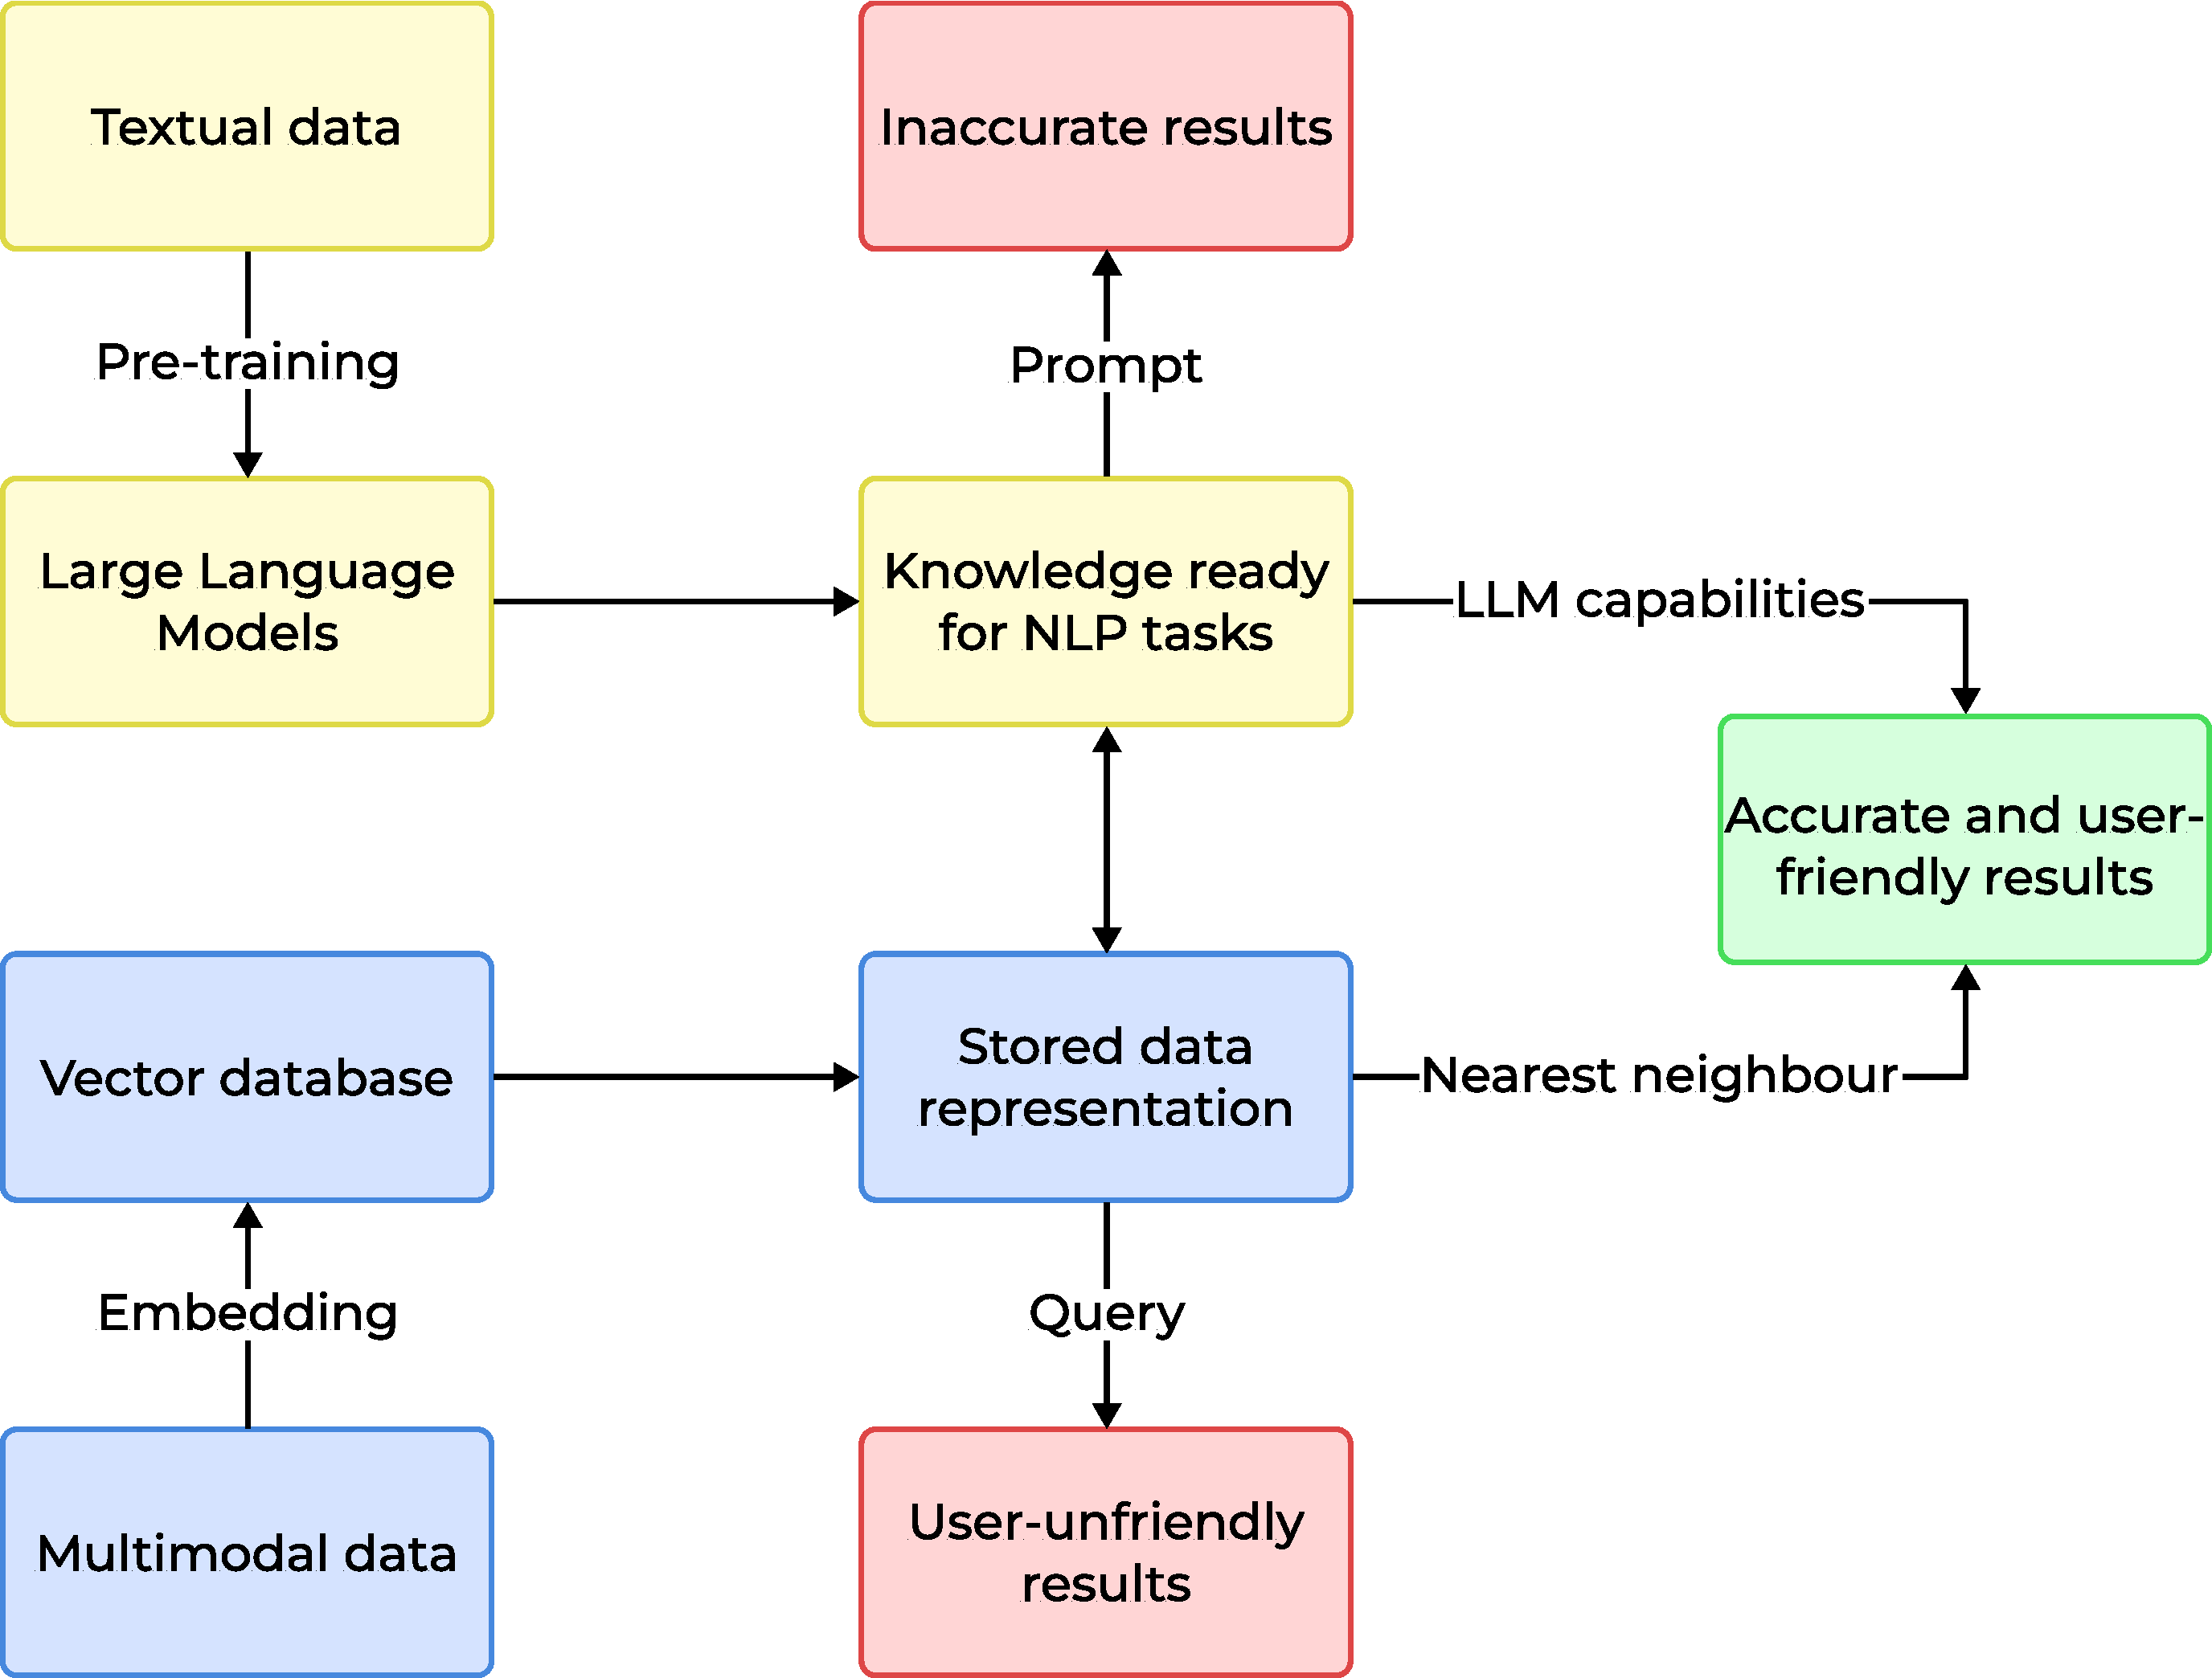
\includegraphics[width=0.9\linewidth]{obrazky/vdbandllm.pdf}
    \caption{Kombinace vektorových databází s velkým jazykovým modelem vzájemně vyvažuje nedostatky jednotlivých přístupů k navracení informací. Převzato z~\cite{compreh_survey_vdb}.}
    \label{fig:vdbandllm}
\end{figure}

Vektorové databáze jsou tak schopny vyhledávat dokumenty relevantní k uživatelskému dotazu a dodávat kontext pro dotazy na generativní modely. Tomuto systému se říká \textit{Retrieval-Augmented Generation} a zaměřuje se na něj zbytek této práce.

\chapter{Retrieval-Augmented Generation (RAG)}
\label{rag}
V publikaci z roku 2021 přišli Lewis et. al. \cite{lewis_rag} se systémem alternativím k čistě parametrizovanému LLM, který by zvýšil přesnost dodávání faktů vyhledáváním informací v externím zdroji. Generování rozšířené o vyhledávání (RAG) je systém, kde \uv{předtrénovaný parametrizovaný generativní model je vybavený neparametrickou pamětí prostřednictvím univerzálního přístupu jemného doladění.}~\cite{lewis_rag}

\section{Limitace velkých jazykových modelů}
RAG kombinuje vyhledávací mechanismy s generativními jazykovými modely pro zvýšení přesnosti výstupů založených na konkrétních faktech. Cílí tak na některé klíčové problémy velkých jazykových modelů.

Většina jich plyne z faktu, že LLM uchovávají svoji paměť v parametrech, na kterých byly natrénovány, tedy v \textit{parametrizované paměti}. Jelikož jsou trénovány na velice rozsáhlém množství dat, dokáží pochytit velké množství znalostí bez využití jakékoliv externí paměti. Jsou též skvělé v generování lidsky vypadajícího textu. Fungují však na základě pravděpodobnosti slovních sekvencí, nikoliv ověřených faktů. Jsou též omezené na data, která byla přítomna ve fázi tréninku~\cite{lewis_rag, compreh_rag}. To vede k určitým limitům:

\begin{itemize}
    \item \textbf{Halucinace}: LLM můžou produkovat odpověď, která sice působí věrohodně, ale je fakticky nesprávná. Může se tak jednat o smyšlené, neexistující informace.
    \item \textbf{Časově omezená znalost}: LLM mají svůj \textit{cut-off date}, tedy datum, kde končí jejich znalosti, typicky datum před trénováním. To vede k tomu, že nemají přístup k aktuálním informacím a jejich znalosti nelze snadno doplnit.
    \item \textbf{Znalosti specifických domén}: LLM jsou typicky obecné modely, a tak jim můžou scházet informace ke specifickým oblastem.
    \item \textbf{Citace}: LLM poskytují své odpovědi bez uvedení zdrojů, to snižuje důveryhodnost a možnosti použití.
    \item \textbf{Soukromá data}: LLM jako obecné modely jsou trénované na veřejně dostupných datech a nemají přístup k soukromým či proprietárním datům.
\end{itemize}

RAG se snaží adresovat tyto problémy přidáním vyhledávacího modulu, který staví na neparametrické paměti~\cite{lewis_rag}. Ta je schopná snadno aktualizovat bázi znalostí, vyhledávat je v reálném čase a poskytovat tak relevantní kontext jako vstup jazykovému modelu společně s uživatelským dotazem. Odpověď je pak srozumitelná, uživatelsky přívětivá a podložena konkrétními dokumenty, které dané fakty uvádějí. Pakliže kontext není dostatečný, je žádoucí aby toto bylo řečeno v odpovědi a je tak vynucena absence smyšlených informací. Báze znalostí pak staví na poskytnutých informacích, které můžou pokrývat specifickou doménu nebo privatní data.

\section{Architektura RAG}
% základní celá flow
Vstupem systému je uživatelův dotaz. Dále RAG kombinuje 2 klíčové komponenty. První je \textit{retriever}, mechanismus vyhledávání infromací v externím úložišti znalostí. Na základě dotazu vyhledává nejrelevantnější informace, které potenciálně obsahují odpoveď. Sada vrácených informací z dokumentů pak tvoří kontext. Ten je společně s uživatelským dotazem formulován jako vstup \textit{generátoru}, který poskytuje uživateli odpověď.

\begin{figure}[H]
    \centering
    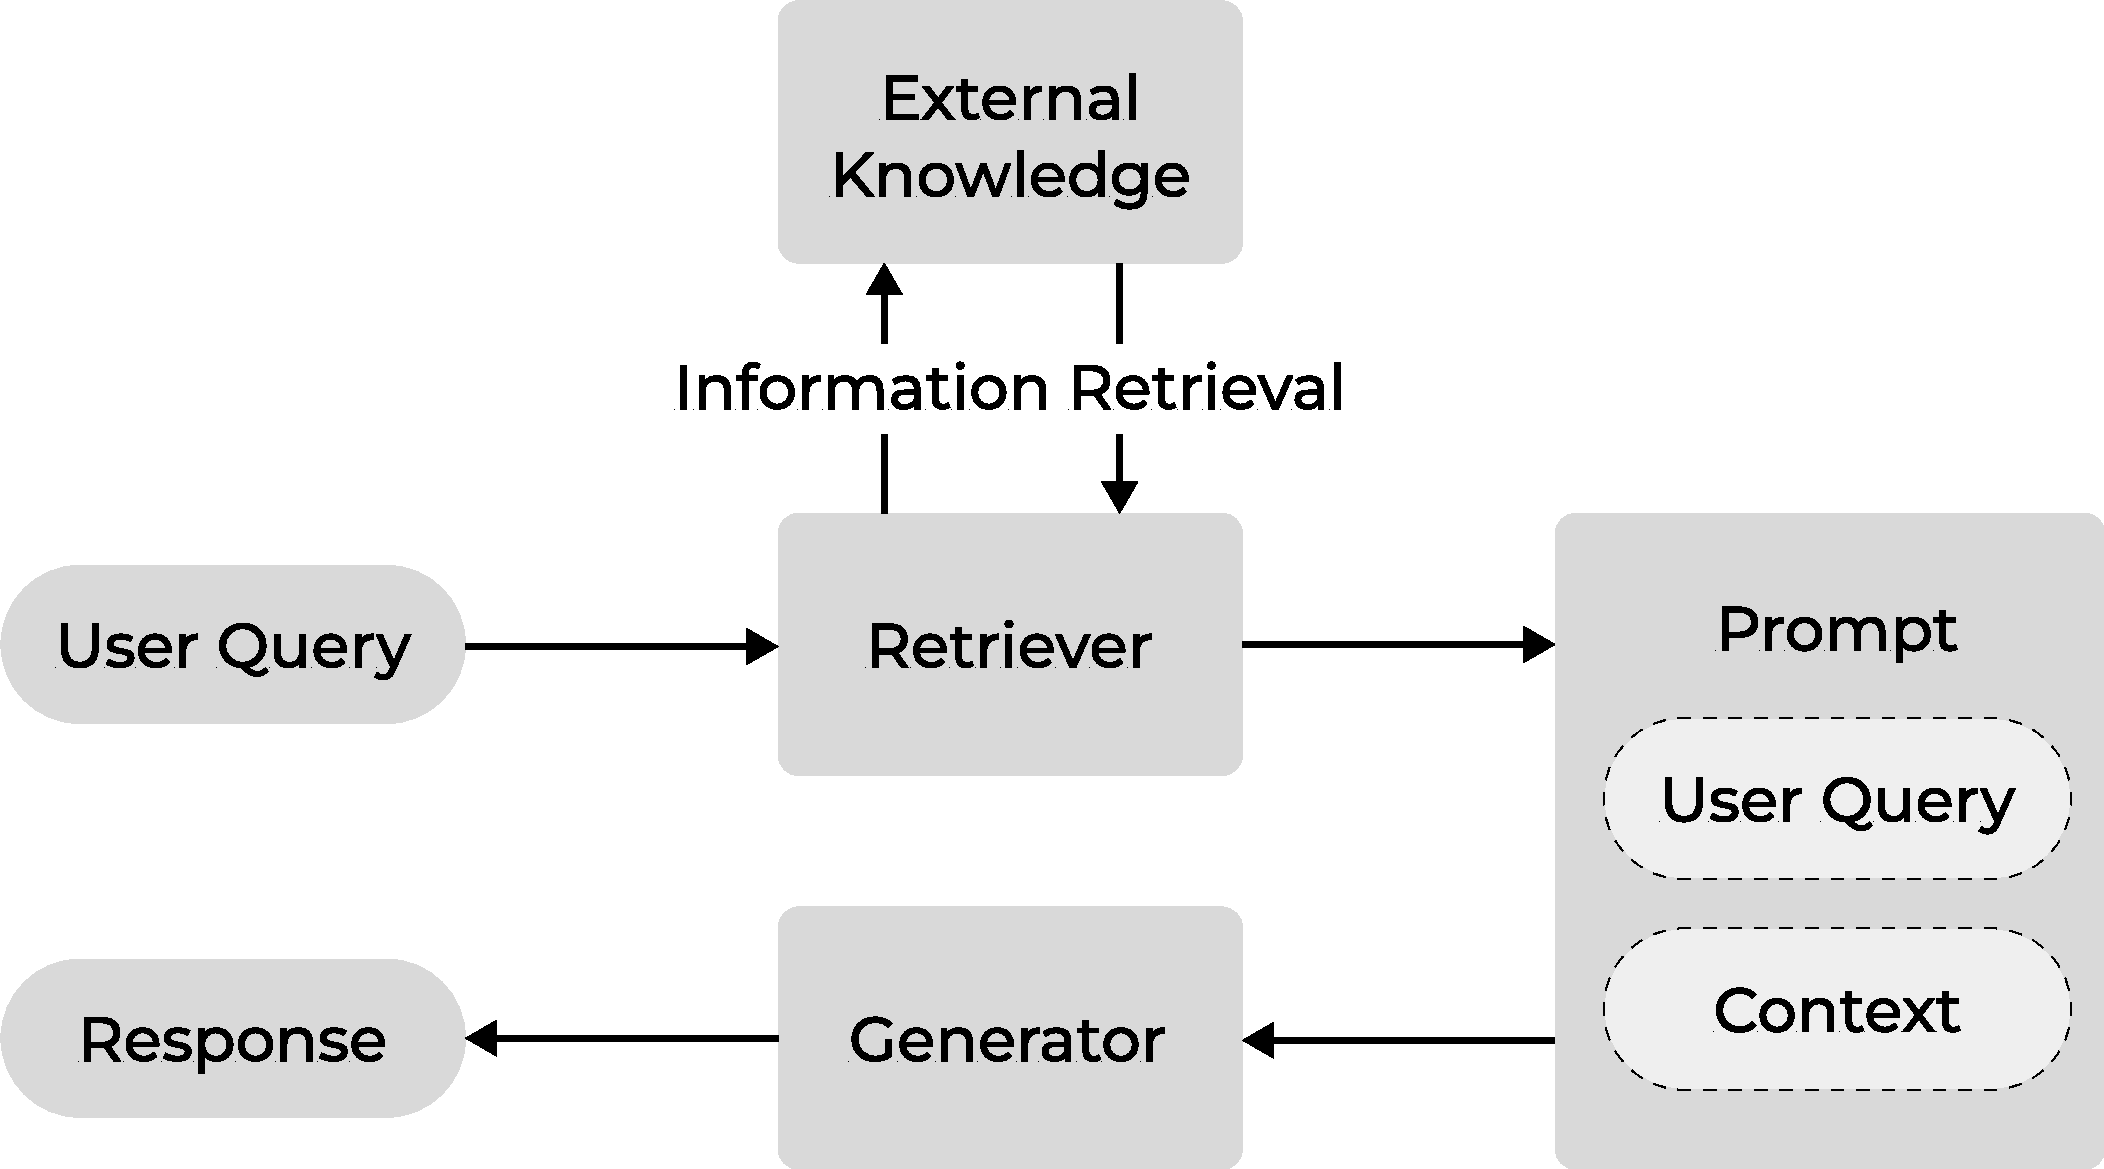
\includegraphics[width=0.7\linewidth]{obrazky/rag.pdf}
    \caption{Základní diagram komponent}
    \label{fig:komponenty}
\end{figure}

% moduly:
% - retriever: dense, sparse (DPR, BM25)
% - generator: LLM
% rag enhancements

\subsection{Retriever}
Retriever je klíčovým modulem systému, který slouží jako nadstavba generátoru a tvoří základ principu Retrieval-Augmented Generation. Jeho hlavním cílem je identifikace relevantních dokumentů nebo jejich částí, které následně slouží jako kontext pro generativní model. Aby systém fungoval v reálněm čase, musí retriever poskytovat výsledky s nízkou latencí, což vyžaduje efektivní indexaci dat (viz \ref{index}) v předzpracovací fázi, tedy vhodnou organizaci dokumentů. Optimalizované algoritmy indexace pak umožňují rychlé vyhledávání i nad rozsáhlými datovými sadami.

Vyhledávání v retrieveru je typicky realizováno pomocí řídkých (\textit{sparse}) nebo hustých (\textit{dense}) vektorových reprezentací. \newpage

\textbf{Řídké vektory} mají vysokou dimenzionalitu a obsahují převážně nulové složky, přičemž nenulové hodnoty obvykle reprezentují váhu nebo frekvenci výskytu termínů v dokumentu. Jsou založeny na metodách tradičního vyhledávání informací pomocí klíčových slov, kde podobnost závísí na přesné shodě termínů. Nejpoužívanějšími metodami jsou:
\begin{itemize}
    \item \textbf{TF-IDF} (\textit{Term Frequency–Inverse Document Frequency}), která vyjadřuje důležitost slova na základě jeho četnosti výskytu v dokumentu~\cite{buttcher2010information},
    \item \textbf{BM25} (\textit{Best Match 25}), pravděpodobnostní model relevance, který kombinuje frekvenci výskytu slov a normalizaci délky dokumentu k odhadu skóre relevance mezi dotazem a dokumenty. Jedná se o jeden z nejrozšířenějších algoritmů pro full-textové vyhledávání \cite{robertson2009bm25}.
\end{itemize}

\textbf{Husté vektory} naproti tomu většinou nulové složky neobsahují a využívají neuronové sítě k mapování dotazů a dokumentů do vektorového prostoru s nižší dimenzionalitou. Takové vektory pak dokáží zachytit i sémantické podobnosti (pomocí nejbližších sousedů) namísto přesné shody termínů, dosahují tak mnohem vyšší výkonnosti než full-textové metody, jsou však výpočetně náročnější a vyžadují embedding modely. Modelem této kategorie pak je \textbf{DPR} (\textit{Dense Passage Retriever}), který používá dva nezávislé transformátorové enkodéry BERT pro mapování dotazu a dokumentu po částech do hustého vektorového prostoru, kde probíhá sémantické vyhledávání porovnáváním dotazu s pasážemi pomocí skalárního součinu~\cite{karpukhin2020dense}.

\subsection{Generátor}
Generativní modul na základě kontextu z navrácených informací a vstupního dotazu produkuje odpovědi ve formě přirozeného jazyka. K tomuto úkolu lze využít kterýkoliv model architektury enkodér-dekodér používané v \textit{seq2seq} transformerových modelech~\cite{murel2024encoderdecoder}. Tento modul je však obvykle implementován pomocí velkého jazykového modelu (LLM). Nejčastěji se využívají transformerové modely jako BART~\cite{lewis2019bart}, T5~\cite{raffel2020T5} nebo GPT~\cite{gpt}, které dosahují nejlepších výsledků v generování přirozeného jazyka.

\subsection{Vylepšení}
Zhao P. et al. ve své práci~\cite{rag_for_aigc} navrhují metody k optimalizaci výsledků pro jednotlivé části RAG, které můžou vést k lepší přesnosti vyhledávání a zlepšení kvality generovaných výsledků. Mezi ty nejpodstatnější v jednotlivých oblastech patří:

\begin{enumerate}
    \item \textbf{Vstup}: Vstupem je uživatelský dotaz a ten ovlivňuje kvalitu výsledku vyhledávání.
    \begin{itemize}
        \item \textbf{Transformace dotazu} – transformace dotazu do optimalizované podoby pro vyhledávání (např. dekompozice komplexního dotazu do více poddotazů).
        \item \textbf{Rozšíření dat} – odstranění nerelevantních informací, dynamická aktualizace dokumentů a přidávání nových.
    \end{itemize}
    
    \item \textbf{Retriever}: Kvalita odpovědi v RAG systémech závisí na relevanci vyhledaných informací, které jsou následně podány generátoru.
    % ADD: limitace - kvalita externich dat
    \begin{itemize}
        \item \textbf{Rekurzivní vyhledávání} – vícenásobné vyhledávání pro zpřesnění nalezeného kontextu.
        \item \textbf{Optimalizace chunkování} – optimalizace velikosti chunků (menších částí dokumentu) pro efektivnější vyhledávání.
        \item \textbf{Doladění retrieveru} – retriever spoléhá na embedding model, který vytváří vektorové reprezentace dat. Kvalita embedding modelu lze doladit pro specifické oblasti informací ke zlepšení sémantického vyhledávání.
        \item \textbf{Hybridní vyhledávání} – použití různých metod vyhledávání (např. kombinace vektorového a fulltextového vyhledávání) nebo získávání informací z více různých zdrojů.
        \item \textbf{Re-ranking} – změna pořadí nalezených dokumentů na základě přezkoumání relevance.
        \item \textbf{Filtrování metadaty} – filtrování dokumentů na základě metadat.
    \end{itemize}
    
    \item \textbf{Generátor}: Kvalita výstupní odpovědi závisí na generátoru při zpracování vstupního kontextu s dotazem.
    \begin{itemize}
        \item \textbf{Prompt engineering} – optimalizace vstupních instrukcí a integrace s navrácenými informacemi.
        \item \textbf{Dolaďení generátoru} – ladění parametrů generativního modelu pro zvýšení kvality odpovědí.
    \end{itemize}

    \item \textbf{Výstup}: Zlepšení celého procesu RAG produkujícího výsledek pak spočívá v identifikaci případů, zdali se vyhledáním skutečně dojde k lepšímu výsledku. Může se stát, že navrácený kontext je pro dotaz nedostatečný. V takových případech je třeba předat zodpovědnost zpět generativnímu modelu, nebo ho v rámci prevence halucinací instruovat, aby neodpovídal bez informací, které by odpověď podložily.
\end{enumerate}

\section{Evaluace RAG systémů}
\label{evaluaceteorie}

Hodnocení kvality RAG systémů není jednoduchý proces kvůli jejich vícevrstvé architektuře a závislosti na externích zdrojích informací. Další komplikací při evaluaci RAG systémů je skutečnost, že generativní model (LLM) zde funguje jako \textit{black-box}. Výsledky, jež produkuje, nemusí být plně transparentní a deterministické. Vyhledávání navíc přímo ovlivňuje kvalitu odpovědí generativního modulu, proto je potřeba testovat jak samostatné moduly, tak RAG jako celek. Pro praktické využití RAG systémů tyto skutečnosti pozdvihují důležitost zavedení automatických vyhodnocovacích postupů, metrik a testovacích sad, které adresují reálné případy použití~\cite{yu2025evaluationrag}.

\subsection{Jednotný proces hodnocení}
V průzkumu nástrojů a benchmarků na evaluaci RAG systémů Yu et. al.~\cite{yu2025evaluationrag} navrhli jednotný proces hodnocení RAG (\textit{Auepora – A Unified Evaluation Process of RAG}), který pomáhá pochopit složitost srovnávacího hodnocení (\textit{benchmarkování}) RAG a vychází z něj tato podkapitola. Auepora je zaměřena na zodpovězení 3 klíčových otázek:
\begin{enumerate}
    \item Co hodnotit?
    \item Jak to hodnotit?
    \item Jak to měřit?
\end{enumerate}

\subsubsection{Cíl hodnocení}
\label{targets}
Základ tvoří 5 cílů hodnocení, které testují jednotlivé vlastnosti RAG systémů. Definují je kombinace výsledků a referenčních základních pravd (tzv. \textit{ground truths}), které jsou předem dané. Určují tak požadavky na RAG systémy.

\begin{figure}[H]
    \centering
    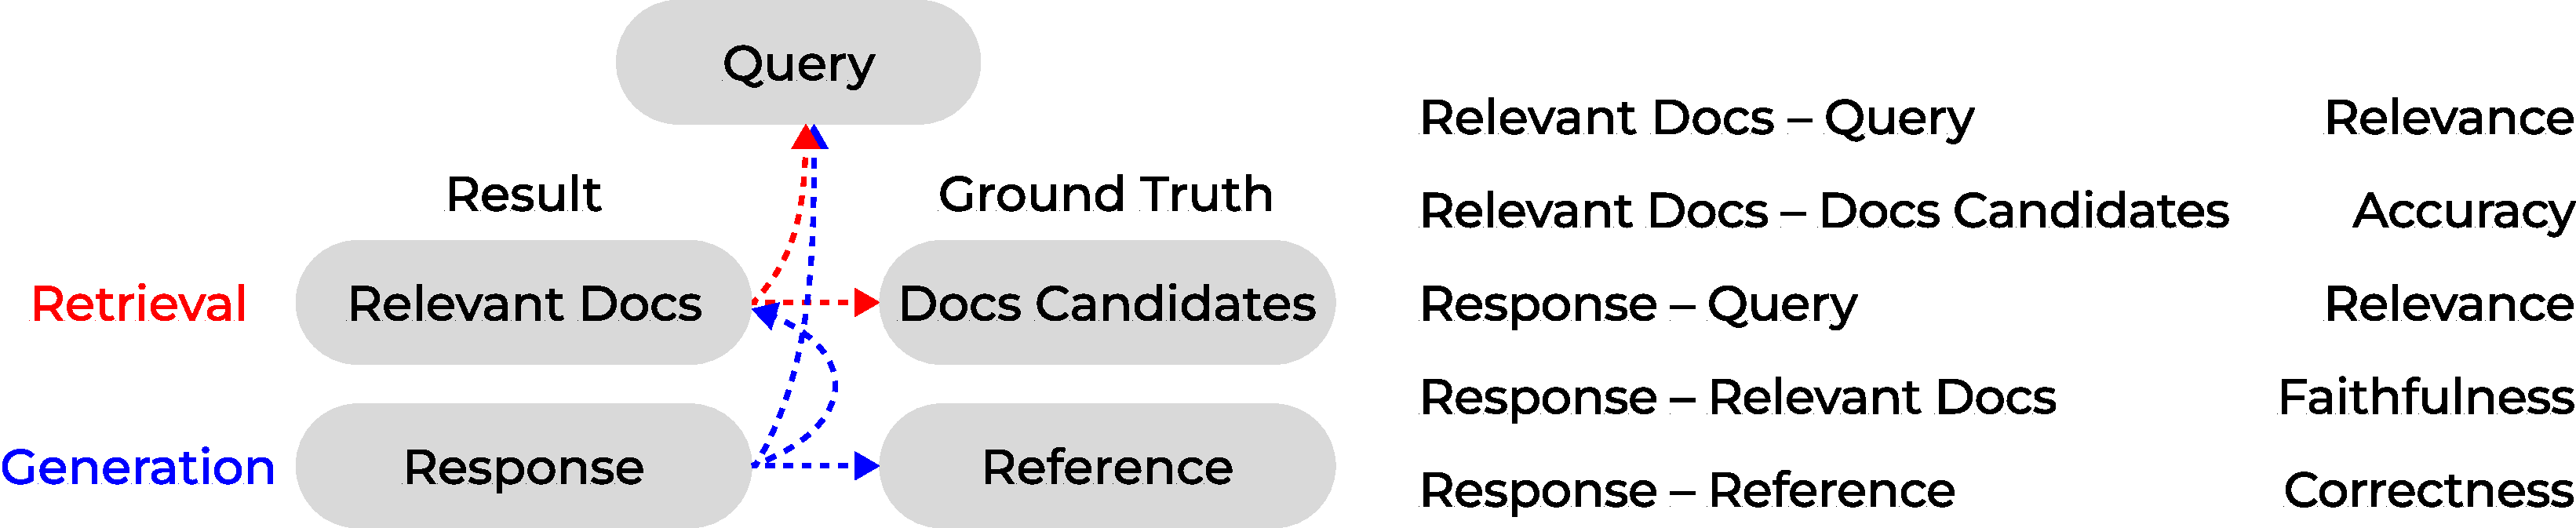
\includegraphics[width=1\linewidth]{obrazky/target.pdf}
    \caption{Diagram možností, které vytváří cíle hodnocení. Převzato z~\cite{yu2025evaluationrag}.}
    \label{fig:targets}
\end{figure}

\begin{enumerate}
    \item Vyhledávání
    \begin{itemize}
        \item \textbf{Relevance} – Určuje, jak dobře vyhledané dokumenty odpovídají vstupnímu dotazu. Cílem je zjistit, zdali systém navrací dokumenty obsahující potřebné informace. 
        \item \textbf{Přesnost} – Porovnává vyhledané dokumenty se sbírkou určených kandidátních dokumentů a tím měří schopnost systému identifikovat relevantní dokumenty včetně jejich priotitizace před méně relevantímí.
    \end{itemize}
    \item Generování
    \begin{itemize}
        \item \textbf{Relevance} – Určuje míru relevance výstupní odpovědi k dotazu, tedy nakolik je vygenerovaná odpověď v souladu se záměrem a obsahem původního dotazu. Zajišťuje, že odpověď souvisí s tématem dotazu a splňuje jeho specifické požadavky.
        \item \textbf{Věrnost} – Hodnotí, zda odpověď vychází z informací obsažených v kontextu z vyhledaných dokumentů.
        \item \textbf{Správnost} – Měří přesnost mezi vygenerovanou odpovědí a odpovědí referenční, která obsahuje ověřené pravdivé tvrzení. Tím je možno pozorovat, zdali je systém schopen dodávat fakticky správné odpovědi mířené na kontext dotazu.
    \end{itemize}
    \item Další požadavky
    \begin{itemize}
        \item \textbf{Latence} – Rychlost vyhledávání a produkce odpovědi, která je nezbytná pro uživatele komunikujícího se systémem.
        \item Zbylé požadavky vychází z benchmarku RGB~\cite{chen2023benchmarkinglargelanguagemodels}:
        \item \textbf{Odolnost proti šumu} – Šum představují dokumenty relevantní otázce, avšak neobsahující správnou odpověď.
        \item \textbf{Odmítnutí} – Aby se předešlo halucinacím LLM, RAG by měl odmítnout odpovědět, pakliže obdržený kontext není dostatečný k poskytnutí odpovědi.
        \item \textbf{Odolnosti vůči protichůdným informacím} – Generátor by měl identifikovat protichůdné fakta ve vyhledaných dokumentech.
    \end{itemize}
\end{enumerate}

\subsubsection{Soubor dat k evaluaci}
K vytváření testovacích případů k hodnocení RAG systémů je klíčový výběr vhodného souboru dat. V popisech některých existujících benchmarků jsou využívané specifické datasety, obecně je však vhodné použít např. index Wikipedie díky její rozmanitosti témat a rozsáhlosti článků. Ověřeným přístupem též je využití sady zpráv o aktualitách. Taková data představují informace, na kterých jazykové modely nebyly trénovány a zodpovědnost tak je plně na vyhledávacím modulu~\cite{yu2025evaluationrag}.

\subsubsection{Metriky hodnocení}
Cíle hodnocení uvádí požadavky na systém. Vytvoření hodnotících kritérií, která by odpovídala lidským preferencím a řešila praktické otázky, je náročné. Existuje však již několik evaluačních frameworků, které implementují řadu metrik, díky kterým je hodnocení měřitelné.

Hodnocení samotných výsledků není vždy deterministické, protože některé metriky, jako například relevance odpovědi k dotazu či věrnost vůči zdrojovým dokumentům, mohou mít subjektivní charakter a závisí na interpretaci hodnotitele. Manuální hodnocení je však časově náročné a často subjektivní. Moderním přístupem k automatizované evaluaci je koncept \textit{LLM-as-a-Judge}~\cite{gu2025surveyllmasajudge, li2024llmsasjudgescomprehensivesurveyllmbased}, kde je jazykový model instruován k ohodnocení relevance, věrnosti či kvality na bodové škále. Tento přístup využívá mimojiné framework popsaný v následující podkapitole, který byl zároveň využit k evaluaci implementovaného RAG systému této práce. 

\subsection{RAGAs: Automatizovaná evaluace RAG systémů}
\label{ragastheory}
Systém RAGAs (\textit{Retrieval Augmented Generation Assessment})~\cite{es2023ragasautomatedevaluationretrieval} předkládá soubor metrik, které lze použít k automatizovanému hodnocení RAG systémů bez nutnosti lidské anotace (poskytnutí referenčních odpovědí). Zároveň využívá vhodné instruování LLM k dělání rozhodnutí, na základě kterých je vypočítáno skóre, vyčísleno od 0 do 1. Níže uvedené metriky vychází z cílů hodnocení uvedených v kapitole~\ref{targets}. Es et. al.~\cite{es2023ragasautomatedevaluationretrieval} pak experimenty dokázali, že pomocí frameworku je dosaženo hodnocení více se shodujícího s hodnocením lidmi, nežli ohodnocení čistě pomocí jazykového modelu.

\subsubsection{Věrnost}
Odpověď je věrná kontextu, pakliže tvrzení uvedená v odpovědi lze odvodit z kontextu. Výstupní odpověď je tak pomocí jazykového modelu rozdělena na jednotlivá tvrzení, kde každé je následně ohodnoceno, zdali souvisí s kontextem.

Výsledné skóre $F$ je vypočteno jako
\begin{equation}
    F = \frac{|V|}{|S|}, 
\end{equation}
kde $|V|$ je počet výroků označených LLM jako podložené kontextem a $|S|$ je celkový počet tvrzení.

\subsubsection{Relevance odpovědi}
Odpověď je relevantní, pakliže se vztahuje ke vstupní otázce. Vygenerovaná odpověď zde slouží jako vstup jazykovému modelu, který generuje otázky k dané odpovědi. Otázky jsou pak embedding modelem převedeny na vektory a je vypočtena vzájemná podobnost mezi původní otázkou a těmi vygenerovanými.

Výsledné skóre $AR$ je vypočteno jako 
\begin{equation}
    AR = \frac{1}{n} \sum_{i=1}^{n} \operatorname{sim}(q, q_i),
\end{equation}
kde $sim(q, q_i)$ je kosinová podobnost mezi původní a vygenerovanou otázkou a $n$ je počet vygenerovaných otázek.


\subsubsection{Relevance kontextu}
Kontext je relevantní, pakliže obsahuje informace potřebné k zodpovězení dotazu. Z kontextu jsou pomocí LLM extrahovány věty, které jsou relevantní k zodpovětení dotazu. Výsledné skóre je vypočteno jako poměr počtu extrahovaných vět a celkovému počtu vět v kontextu.

\section{Aplikace}
% openQA, domain-specific, company, 

% -> OpenQA
% In simple terms, RAG is to LLMs what an open-book exam is to humans. In an open-book exam, students are allowed to bring reference materials, such as textbooks or notes, which they can use to look up relevant information to answer a question. The idea behind an open-book exam is that the test focuses on the students’ reasoning skills rather than their ability to memorize specific information.

% https://towardsdatascience.com/retrieval-augmented-generation-rag-from-theory-to-langchain-implementation-4e9bd5f6a4f2/
% Retrieval-Augmented Generation (RAG) nachází široké uplatnění v situacích, kde je třeba poskytovat odpovědi založené na rozsáhlých, často interních datech, která nejsou součástí tréninkové sady jazykového modelu. V této sekci jsou popsány praktické scénáře využití RAG a ilustrováno konkrétní nasazení v rámci systému implementovaného v této práci.

% \subsection{Open-Domain Question Answering (OpenQA)}
% RAG je často využíván v tzv. \textit{Open-Domain Question Answering}, kde cílem je zodpovědět dotaz pomocí rozsáhlé a potenciálně otevřené báze znalostí (např. Wikipedia). Na rozdíl od klasických LLM, které si musí vystačit s vlastními parametry, má RAG schopnost dynamicky získávat aktuální informace, což výrazně zlepšuje faktickou správnost odpovědí. Tento přístup se často přirovnává k „open-book testu“ pro jazykové modely, kdy mají k dispozici dokumenty jako zdroj faktů během odpovědi.

% \subsection{Doménově specifické systémy}
% Další důležitou aplikací je vyhledávání v doménově specifických dokumentech. Může jít o interní firemní dokumentaci, manuály, právní předpisy nebo vědecké články. V těchto scénářích je RAG využíván k získávání odpovědí v oblasti, kde standardní LLM selhávají kvůli nedostatečnému pokrytí v trénovacích datech.


%------------------------------------------------------------------------------------------------
%------------------------------------------------------------------------------------------------
%------------------------------------------------------------------------------------------------

\chapter{Architektura systému}
\label{navrh}
% diagram architektury a popis interakce mezi jednotlivými komponentami
Předchozí kapitoly shrnují dosažený vědecký pokrok v oblastech vektorových databází a Retrieval-Augmented Generation. Slouží tak jako teoretický základ, který vytvořil kontext pro použití těchto technologií k návrhu a implementaci vlastního systému na zpracování a vyhledávání dokumentů. 

Tato kapitola si dává za cíl představit architekturu systému, který vznikl v rámci této práce. Principem vychází z přístupu RAG. Hlavní myšlenkou je dotazování systému, který odpovídá na otázky pomocí externího zdroje informací (na bázi Q\&A). Zdroj informací zde představují textové dokumenty propojené se systémem, které jsou uložené ve vektorové databázi. Jedná se tak o vyhledávání nad těmito dokumenty, přičemž otázka je podána přirozeným jazykem a odpověď je uživatelsky přívětivá, podložená fakty s odkazy na zdroje infromací. Využití systému není nijak limitováno, záleží pouze na tom, jaká data na textové bázi má systém k dispozici.

Systém je navrhnut tak, aby optimalizoval přesnost vyhledávání, která je nutná pro formulaci správné odpovědi generátorem. Vyhledávání informací z dokumentů je cílové použití, jedná se však až o druhou fázi. První fází systému je zpracování dokumentů a jejich uložení do databáze. 


\section{Zpracování dokumentů}
\label{zpracovani}
Prvním procesem je zpracování dokumentů. Vstupem je dokument, který je konvertován na prostý text. Ačkoliv byl systém testován především na textových dokumentech, podporovanými typy souborů jsou \texttt{.txt}, \texttt{.doc}, \texttt{.docx}, \texttt{.pdf}, \texttt{.jpg}, \texttt{.png} a \texttt{.heic}. Na binární soubory, jako jsou obrázky a PDF dokumenty, se aplikuje OCR (optické rozpoznávání znaků) k extrakci textu. Extrahovaný text prochází předzpracováním, které zahrnuje čištění textu a případnou detekci nadpisů. Dále je rozdělen na tzv. chunky, které představují kratší pasáže textu. To vše je úkol modulu \texttt{DocumentProcessor}. 


Každý chunk je obohacen o metadata zahrnující informace o dokumentu, ze kterého textová pasáž pochází, a pro snadnější lokalizaci i ve které sekci nebo na které straně se nachází. Dále obsahuje údaje o přístupových právech k dokumentu, které umožňují filtrování. 

Jakmile jsou dokumenty rozděleny na chunky a obohaceny o metadata, dalším krokem je jejich vektorizace. Text každého chunku je převeden do vektorové reprezentace pomocí embedding modelu. Ty jsou přidány k chunkům, které se ukládájí do vektorové databáze.

\begin{figure}[H]
    \centering
    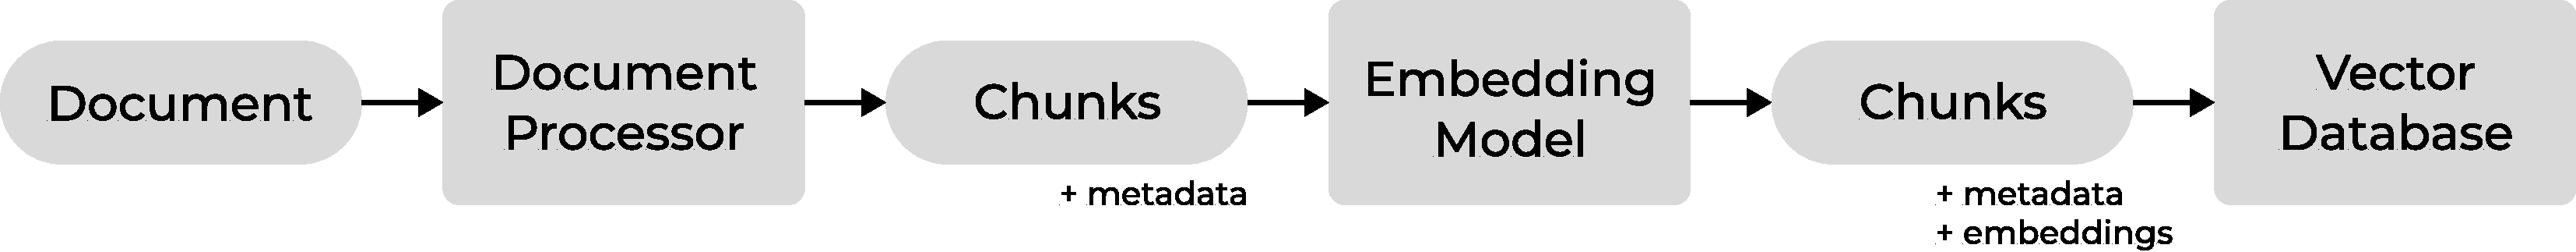
\includegraphics[width=1\linewidth]{obrazky/processing.pdf}
    \caption{Diagram zpracování dokumentu až po jeho uložení do databáze}
    \label{fig:zpracovani}
\end{figure}

\subsection{Chunking}
\label{chunking}
Chunking je proces dělení textu na sekce velikostně optimalizované pro zpracování jazykovými modely a zachycení kontextu. Zatímco dokumenty jsou většinou příliš velké a zahrnují široký, mnohdy různorodý kontext, chunking dělí dokumenty na logické sekce zachycující jeden kontext, které jsou navíc velikostně přizpůsobené vektorizaci embedding modelem, který má svůj limit.

Strategie chunkingu se dělí podle komplexnosti. Naivním přístupem je dělení textu na bloky o fixní délce, to však může rozdělit jeden kontext do více pasáží, navíc i uprostřed slova. Rekurzivní přístup pak dělí text podle struktury (odstavce, nadpisy, věty) a dodržuje limit velikosti chunku.

Metoda, kterou systém implementuje, se snaží co nejvíce zachovat kontext a strukturu textu, přičemž velikost chunku omezuje vstupní limit embedding modelu. Ten je počítán v tokenech, a proto i text je tokenizérem příslušného embedding modelu přepočítáván na tokeny. Na obrázku~\ref{fig:tokenizer} je zobrazen princip tokenizace\footnote{nástroj dostupný na gpt-tokenizer.dev}.

\begin{figure}[H]
    \centering
    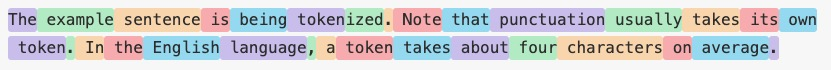
\includegraphics[width=1\linewidth]{obrazky/tokens.jpg}
    \caption{Vizualizace tokenizace}
    \label{fig:tokenizer}
\end{figure}

Dokument je rozdělen na jednotlivé věty, které jsou přidávány do chunku. Pakliže by počet tokenů ve větě přesáhl limit chunku, aktuální chunk se uzavře a věta je přidána do nového chunku společně s poslední větou předchozího chunku. Tím dochází k překryvu, který zabraňuje ztrátě kontextu mezi sousedními částmi textu. Nadpisy pak vždy tvoří počátek nového chunku, protože označují začátek nového logického celku.

\begin{figure}[H]
    \centering
    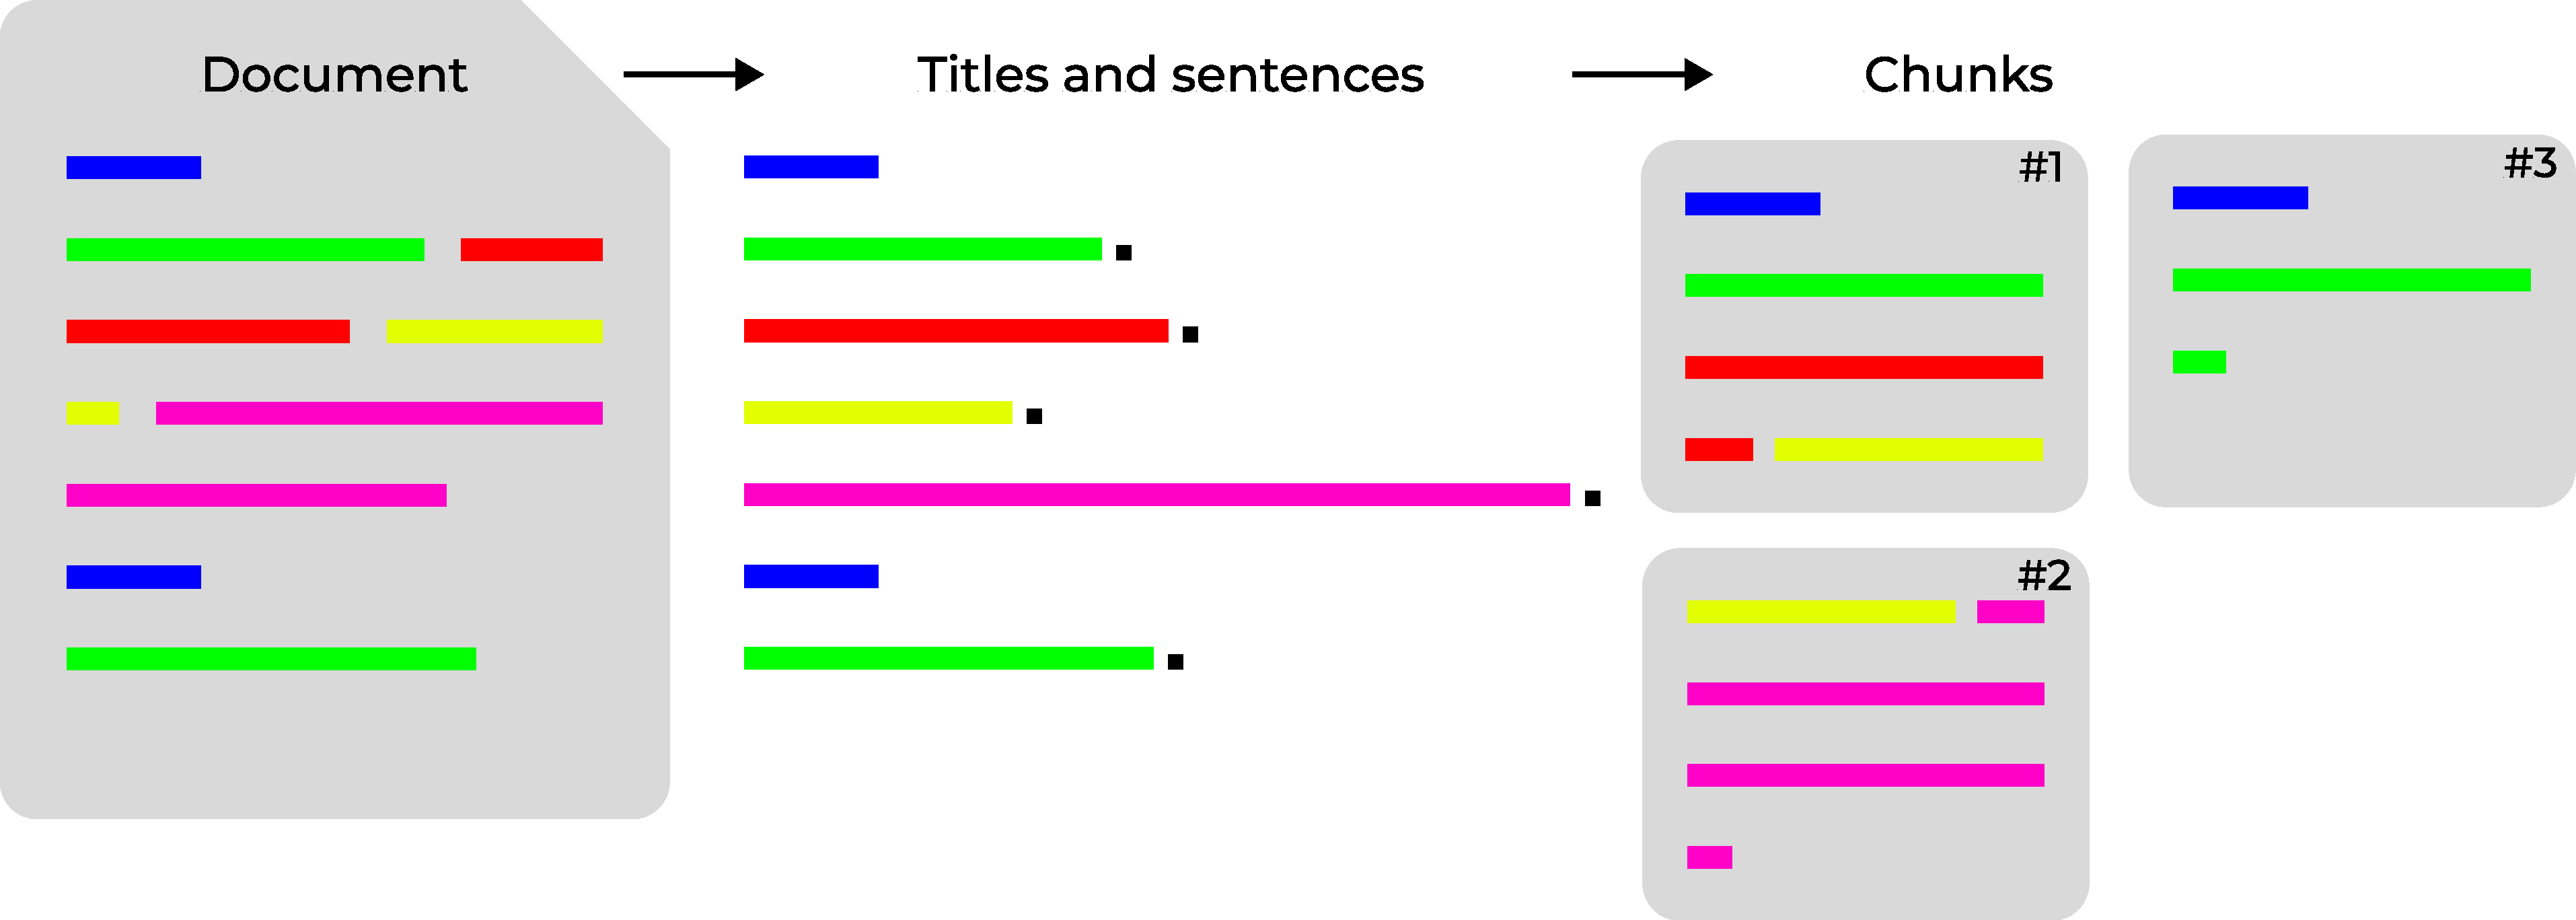
\includegraphics[width=1\linewidth]{obrazky/chunking.pdf}
    \caption{Chunking}
    \label{fig:chunking}
\end{figure}


\section{Vyhledávání dokumentů}
Vyhledávání dokumentů pro vytvoření kontextu a poskytnutí odpovědi formulované jazykovým modelem je hlavním případem užití systému. Jakmile vektorová databáze obsahuje data, která slouží jako báze znalostí, nastává druhá fáze systému. 

Dotaz uživatele je přeformulován do podoby optimalizovanější pro vyhledávání. Přeformulovaný dotaz je použit pro hybridní vyhledávání, které navrací relevantní chunky. Ačkoliv mají své skóre vyhledávání, jejich pořadí a relevance je upřesněna pomocí modulu \texttt{Reranker}. Tyto chunky pak slouží jako kontext pro jazykový model, který pomocí něj zodpovídá dotaz uživatele.

\begin{figure}[H]
    \centering
    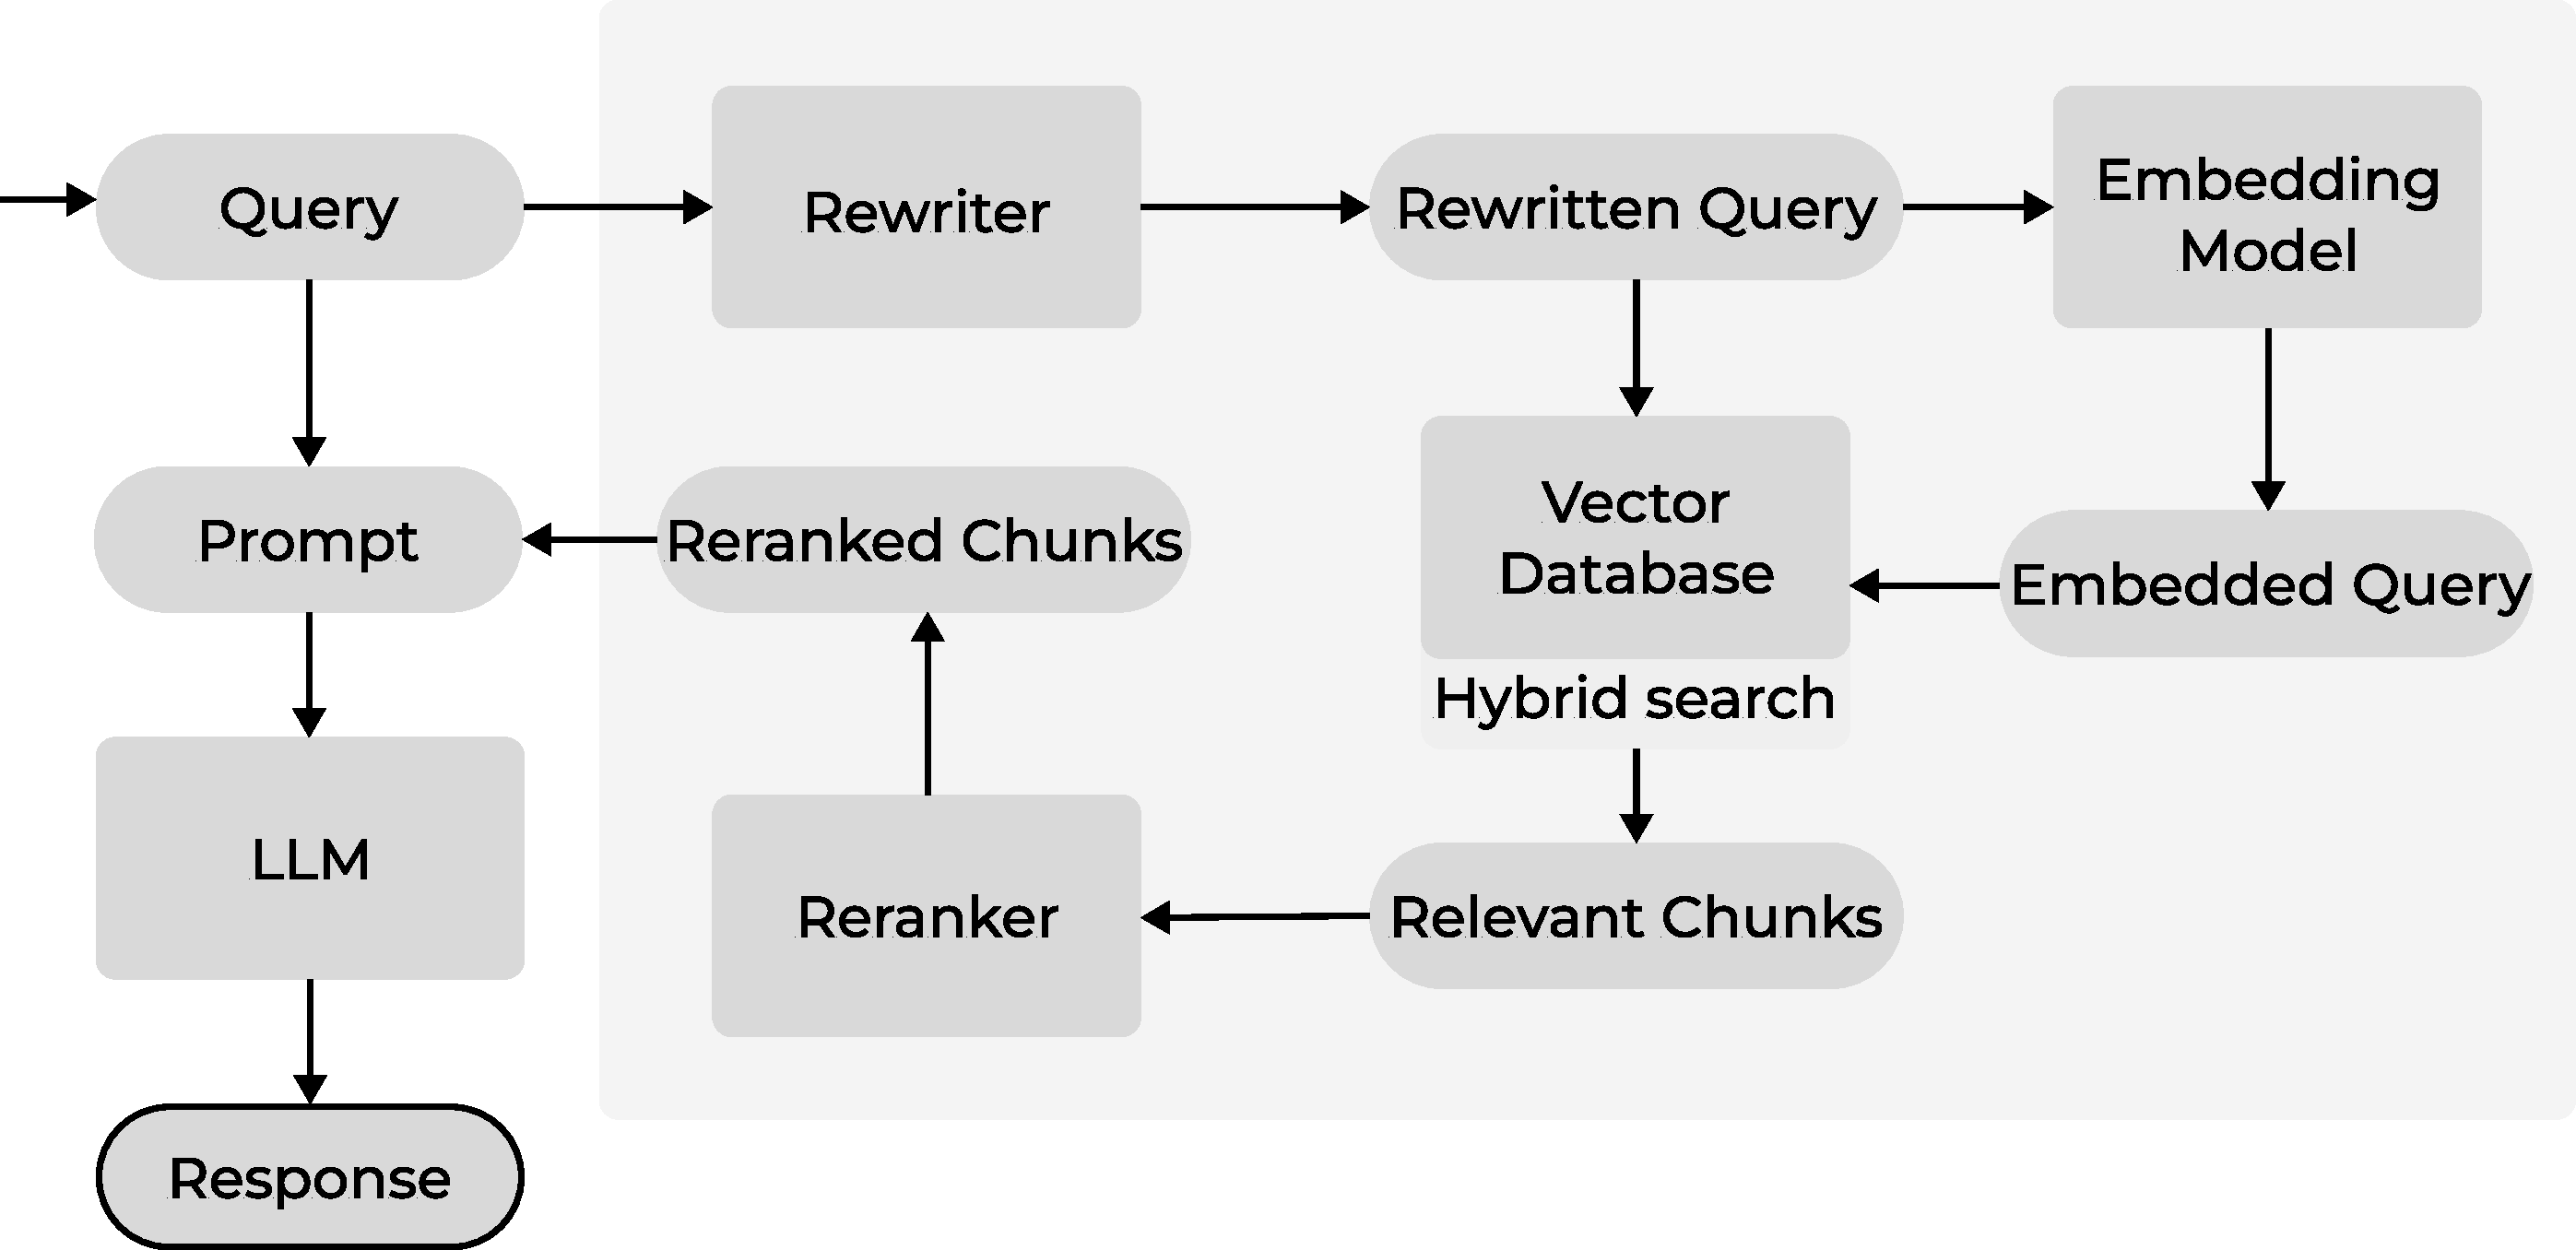
\includegraphics[width=1\linewidth]{obrazky/retrieval.pdf}
    \caption{Diagram komponent vyhledávání dokumentů a generování odpovědi}
    \label{fig:retrieval}
\end{figure}

\subsection{Přeformulování dotazu}
Modul \texttt{Rewriter} má v systému 2 módy. První slouží k optimalizaci dotazů pro vyhledávání. Uživatelé často formulují své dotazy neefektivně tím, že používají nadbytečná nebo vycpávková slova. Při zadávání dotazu uživatelem přes klávesnici navíc může dojít k překlepům, které by mohly negativně ovlivnit výsledek vyhledávání. Tento modul využívá jazykový model a vhodně ho instruuje k přeformulování dotazu do stručnější a informativnější podoby, aniž by změnil jeho původní význam.

\begin{figure}[H]
    \centering
    
\includegraphics[width=0.7\linewidth]{obrazky/rewriting.pdf}
    \caption{Příklad uživatelského vstupu (nahoře), který je pro vyhledávání přeformulován na dotaz \uv{capital of Belgium}, a odpovědi}
    \label{fig:rewriting}
\end{figure}

Klade si tak za cíl zpřesnit obě složky hybridního vyhledávání. U fulltextového vyhledávání je dotaz omezen na relevantní slova a u sémantického vyhledávání vede zjednodušený dotaz k lepší vektorové reprezentaci, která přesněji odpovídá uloženým embeddingům a eliminuje zkreslení způsobené nadbytečnými slovy.



Vhodně formulované dotazy pak ponechává beze změny. V případě nesmyslných nebo nejednoznačných dotazů k přeformulování také nedochází, aby nebyly ovlivněny další fáze vyhledávání, které s těmito případy počítají.

\subsection{Chatová historie}
Druhým módem modulu \texttt{Rewriter} je podpora chatové historie a navazujících otázek. Při zadání neúplného dotazu, který se odkazuje k předešlým otázkám a odpovědím, je tento dotaz s pomocí 3 posledních párů dotaz–odpověď přeformulován jazykovým modelem do kompletní podoby.

\begin{figure}[H]
    \centering
    
\includegraphics[width=0.7\linewidth]{obrazky/chathistory.pdf}
    \caption{Příklad navazující otázky \uv{and germany?}, která je pro vyhledávání i výsledný prompt generátoru přeformulována na dotaz \uv{What is the capital of Germany?}}
    \label{fig:rewriting}
\end{figure}

Tento mód přináší novou funkcionalitu, vykazuje však potenciálně horší výkon systému. Zatímco první mód dotazy zjednodušuje, druhý je obohacuje. Generátoru je podán přeformulovaný dotaz namísto původního, aby na něj byl schopen odpovědět. Při úplných dotazech však může dojít k mírnému přeformulování a nekonzistencí mezi otázkou a odpovědí.

\subsection{Hybridní vyhledávání}
\label{hybrid}
Hybridní vyhledávání kombinuje fulltextové a vektorové vyhledávání k využití obou metod pro přesnější výsledky. Motivací tohoto přístupu je fakt, že dotazy bývají různorodě zaměřené. 
\begin{itemize}
    \item \textbf{Fulltextové vyhledávání} je přesné při hledání konkrétních klíčových slov. Pokud ale uživatel použije synonyma nebo volnější formulaci dotazu, bývá nepřesné. Vstupem fulltextovému vyhledávání je přeformulovaný dotaz.
    \item \textbf{Vektorové vyhledávání} dokáže najít sémanticky podobné výsledky i při odlišné formulaci, ale nemusí vždy zaručit, že nalezené dokumenty obsahují specifická klíčová slova, což může vést k nižší přesnosti u některých dotazů. Vstupem vektorovému vyhledávání je vektorová reprezentace přeformulovaného dotazu, vytvořená stejným embedding modelem, který byl použit ke zpracování dokumentů.
\end{itemize}
Hybridní vyhledávání využívá parametr $\alpha$, který určuje váhu mezi fulltextovým a vektorovým vyhledáváním. Je vyčíslen hodnotou $\alpha \in \langle 0, 1 \rangle$, kde 0 se příklání fulltextovému vyhledávání a 1 vektorovému. 
Výsledné skóre je pak vypočteno jako vážený průměr normalizovaných hodnot skóre jednotlivých vyhledávání:

\begin{equation}
    s_{\text{hybrid}} = \alpha \cdot \frac{s_{\text{vector}} - \min(s_{\text{vector}})}{\max(s_{\text{vector}}) - \min(s_{\text{vector}})} + (1 - \alpha) \cdot \frac{s_{\text{fulltext}} - \min(s_{\text{fulltext}})}{\max(s_{\text{fulltext}}) - \min(s_{\text{fulltext}})},
\end{equation}

kde $s_{\text{fulltext}}$ je skóre z fulltextového vyhledávání (např. BM25) a $s_{\text{vector}}$ je skóre vektorového vyhledávání, které může být založeno např. na kosinové podobnosti nebo Euklidovské vzdálenosti.

\subsection{Reranking}
Tato část vychází převážně ze zdroje \cite{reranking}, kde je proces vyhledávání označen za dvoufázový, protože důležitým krokem po hybridním vyhledávání je tzv. \textit{reranking}. Jedná se o proces přeuspořádání či zpřesnění výsledků původního vyhledávání podle míry relevance k dotazu uživatele.

Samotné vyhledávání často upřednostňuje rychlost před přesností, jelikož probíhá nad rozsáhlým množstvím dat (viz ANNS~\ref{anns}). V této fázi se typicky využívá architektura \textit{Bi-encoder}, kde jsou dotaz a dokument zakódovány odděleně a jejich relevance je určena pomocí podobnostní funkce. Tento přístup je rychlý, ale může u něho docházet ke ztrátě sémantických detailů. Jeho výsledkem je pevně daný počet nejrelevantnějších chunků.

Reranking využívá předtrénovaný model typu \textit{Cross-encoder}, který dotaz a jednotlivé chunky zpracovává společně jako jeden vstup a dokáže tak detailněji zachytit jejich sémantickou souvislost. Každé dvojici dotaz–chunk je přiřazeno skóre relevance, podle kterého jsou výsledky seřazeny. Zároveň provádí filtr tím, že informace s nedostatečnou mírou relevance z kontextu odstraní. Vzhledem k vyšší výpočetní náročnosti se reranking aplikuje pouze na omezený počet chunků, právě proto následuje samotnému vyhledávání.

Výsledkem by měla být vyšší kvalita odpovědi generované jazykovým modelem, protože se do promptu dostávají pouze skutečně relevantní informace a LLM tak není zahlceno přebytečnými informacemi.

\subsection{Prompt Engineering}
Posledním krokem před samotným generováním odpovědi jazykovým modelem je návrh promptu, který pak slouží jako jeho vstup. Cílem \textit{prompt engineeringu} je navrhnout takový vstup, který co nejlépe instruuje model ke správné odpovědi dodržující zamýšlený formát.

Návrh promptů v RAG systémech je zásadní, jelikož model nesmí odpovídat na základě natrénovaných dat, ale musí kombinovat dotaz s poskytnutým kontextem. Dle dokumentace OpenAI~\cite{openaidocs} patří mezi základní principy prompt engineeringu:
\begin{itemize}
    \item \textbf{Využití rolí} – Při jednom volání lze využít více zpráv různé priority, konkrétně \texttt{developer} zpráva typicky obsahuje instrukce a pravidla a má vyšší prioritu, \texttt{user} zpráva pak obsahuje vstup, na který jsou pravidla uplatněna.
    
    \item \textbf{Formátování a struktura promptu} – Pomocí Markdown formátování a XML tagů lze pomoct modelu s pochopením instrukcí a logicky strukturovat prompt. Struktura promptu pak obecně bývá člěněna do sekcí v následujícím pořadí: identita, instrukce, příklady a kontext.
    
    \item \textbf{Identita} – Nastavení identity (mimo samotné instrukce) poskytuje modelu rámec chování a stylu odpovědi, říká mu, jaká je jeho role.

    \item \textbf{Few-shot learning} – Tato metoda poskytuje v promptu pár ukázkových příkladů vstup–výstup, ze kterých si model implicitně vyvodí požadované chování. 

    \item \textbf{Kontext} – Poskytnutí kontextu s relevatními informacemi k zodpovězení dotazu je celý princip Retrieval-Augmented Generation.
\end{itemize}

Prompty mají předdefinované instrukce a následně jsou tvořeny a formátovány dynamicky v kódu na základě dotazu a vyhledaného kontextu. Použité prompty v systému jsou uvedeny v~kapitolách~\ref{rewriter} a \ref{llmwrapper}.

\section{Integrace komponent}
Předchozí podkapitoly uvedly princip dvou hlavních fází systému:
\begin{enumerate}
    \item \textbf{Zpracování}, kde vstupem je textový dokument, který je zpracován a uložen do vektorové databáze.
    \item \textbf{Vyhledávání}, kde vstupem je dotaz uživatele a výstupem je odpověď formulovaná LLM pomocí vyhledaného kontextu.
\end{enumerate}
Tyto fáze se mohou neustále opakovat a společně s integrací cloudového úložiště a webového uživatelského rozhraní tvoří celou architekturu systému. Jednotlivé komponenty lze pak rozdělit podle jejich funkční odpovědnosti na třívrstvou architekturu znázorněnou na obrázku~\ref{fig:three-tier}.

\begin{figure}[H]
    \centering
    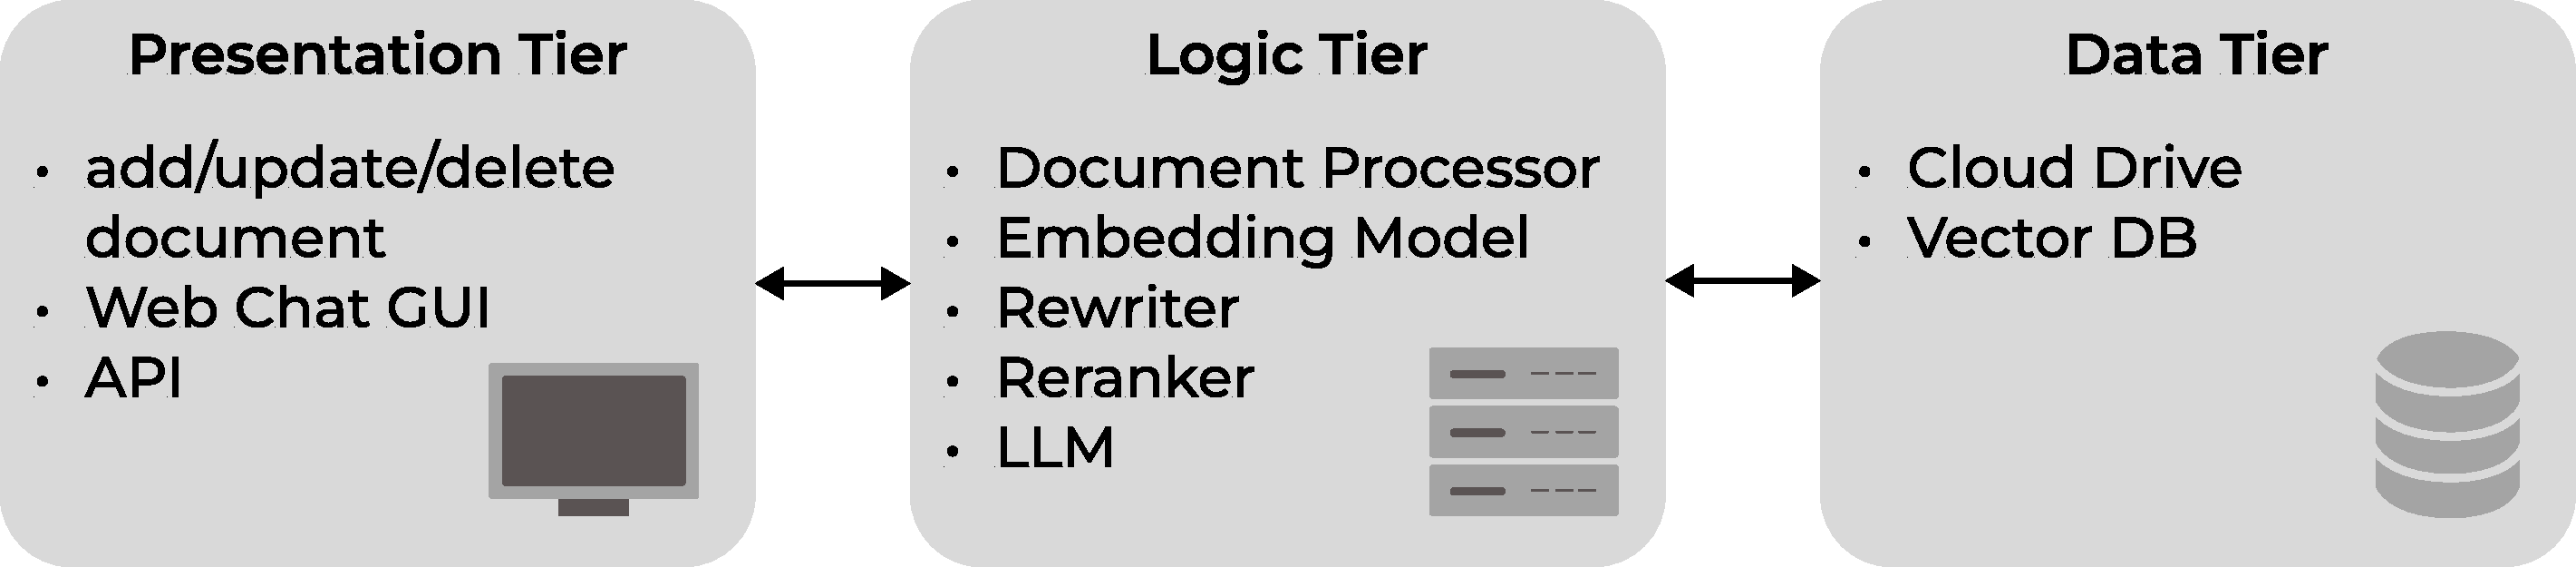
\includegraphics[width=0.9\linewidth]{obrazky/threetier.pdf}
    \caption{Třívrstvá architektura systému}
    \label{fig:three-tier}
\end{figure}

\subsection{Synchronizace s cloudovým úložištěm}

Součástí systému je integrace s cloudovým úložištěm, které slouží pro správu dokumentů tvořících bázi znalostí. Uživatel může dokumenty nahrávat, upravovat nebo mazat ve vyhrazené složce v prostředí cloudové služby, kterou si se systémem propojí. 

Tato složka je systémem monitorována. Jakmile se její stav změní, systém je o tom prostřednictvím API cloudové služby notifikován a zahajuje synchronizační rutinu, která obnáší detekci změn a zajištění jejich promítnutí do databáze.

Při detekci nového dokumentu je tento dokument stažen a prochází fází zpracování. V případě smazání dokumentu jsou příslušné chunky z databáze odstraněny a při detekci změn v již nahraném dokumentu dochází ke kombinaci těchto procesů, tedy smazání a znovuzpracování.

Tímto způsobem je zajištěno, že znalostní báze systému vždy reflektuje aktuální stav cloudového úložiště automatickou synchornizací.

\subsection{Tok dat v systému}

Na obrázku~\ref{fig:flow} je znázorněna celková architektura systému a vzájemné propojení komponent. 

\begin{figure}[H]
    \centering
    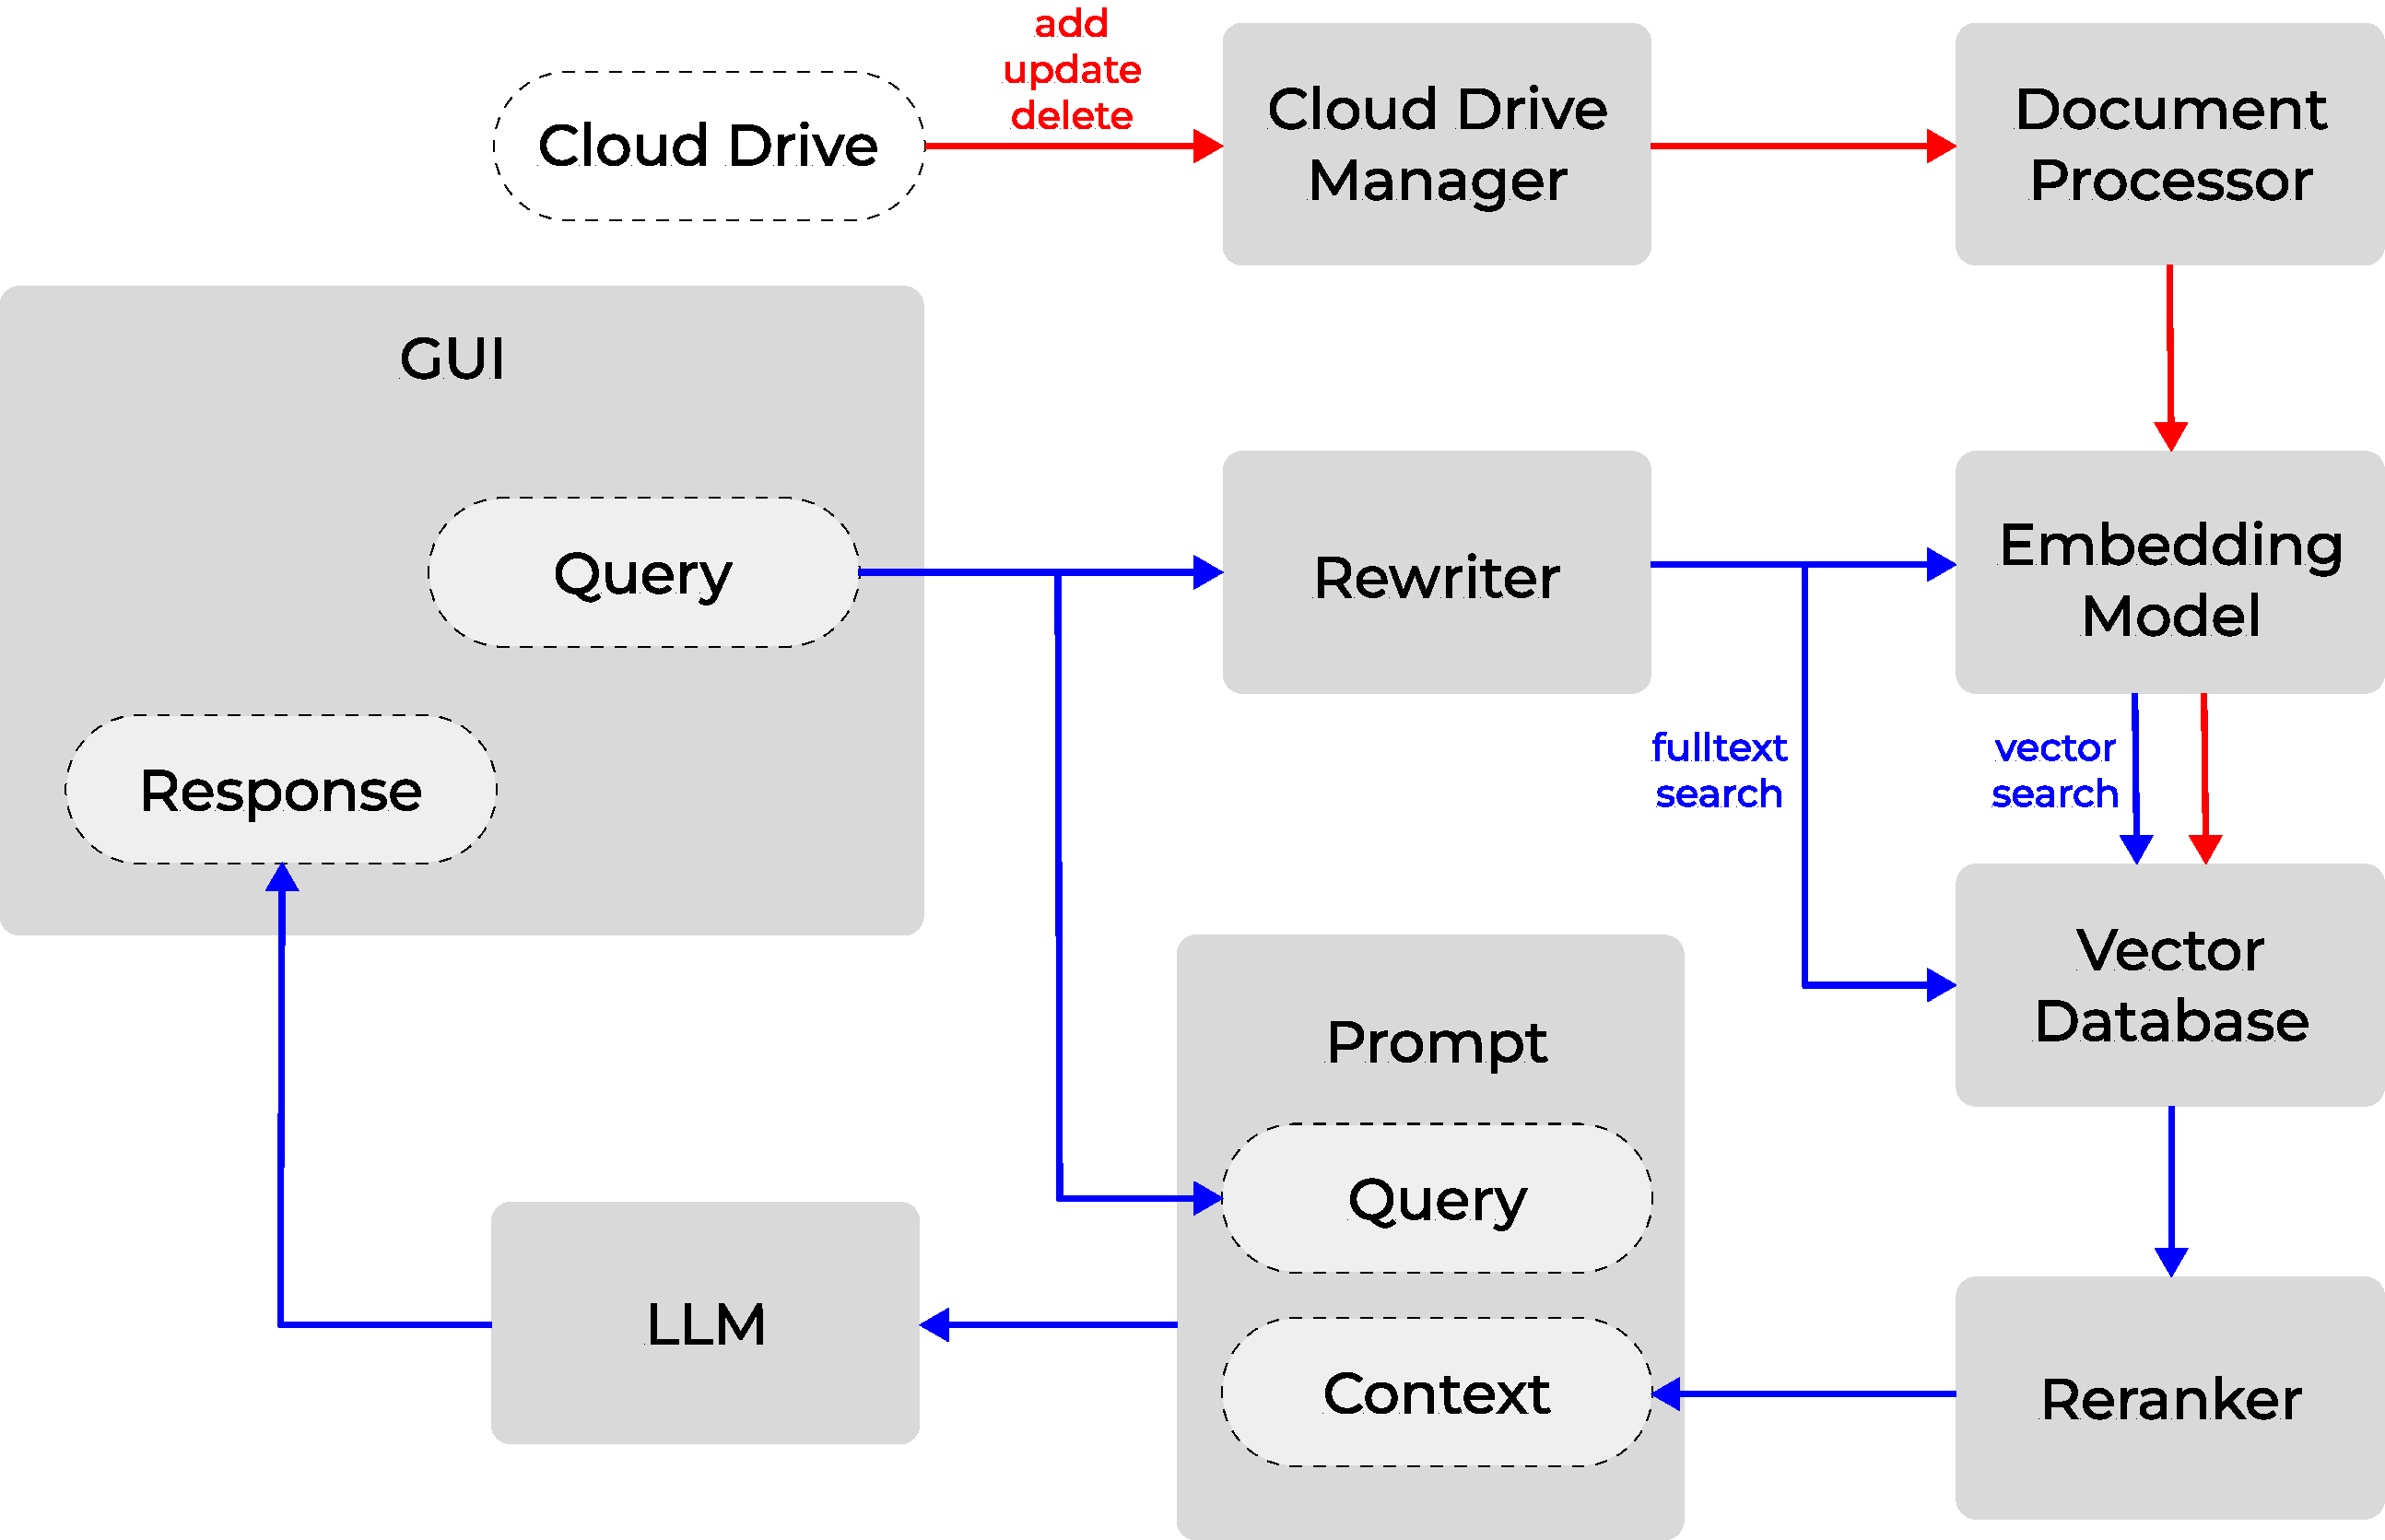
\includegraphics[width=1\linewidth]{obrazky/system.pdf}
    \caption{Diagram komponent}
    \label{fig:flow}
\end{figure}

\chapter{Implementace}
\label{implementace}
Tato kapitola se věnuje technické realizaci systému navrženého v předchozí kapitole. Popisuje především použité technologie, knihovny, modely a jejich výběr. Následuje způsob implementace jednotlivých komponent. Dále je zde vysvětleno, jakým způsobem systém komunikuje s externími službami a jak jsou zajištěny interakce mezi jednotlivými moduly systému a uživatelským rozhraním prostřednictvím API. Při zmínkách použitých technologií u implementačních detailů jsou uvedeny citace k dokumentacím, které byly při implementaci využity.

\section{Použité technologie}
Při implementaci systému byla využita existující řešení pro jednotlivé dílčí úkoly systému, které byly integrovány do funkčního celku Retrieval-Augmented Generation. 

Systém je implementován v jazyce Python. Vývoj a testování systému probíhalo lokálně pomocí technologie Docker Compose, která umožnila spouštění jednotlivých komponent (API server, databáze, frontend) v konzistentním prostředí. Níže je uveden přehled hlavních knihoven a nástrojů, které byly v rámci implementace použity:
\begin{itemize}
    \item \textbf{FastAPI} – webový framework k propojení backendu a frontendu skrze API.
    \item \textbf{Unstructured} – knihovna poskytující rozhraní pro zpracování nestrukturovaných dat.
    \item \textbf{NLTK} (Natural Language Toolkit) – sada knihoven pro zpracování přirozeného jazyka.
    \item \textbf{Transformers} (HuggingFace) – knihovna pro práci s předtrénovanými jazykovými modely, využita pro tokenizér. 
    \item \textbf{Sentence Transformers} (HuggingFace) – nadstavba s modely pro vytváření vektorových reprezentací.
    \item \textbf{Weaviate} – open-source vektorová databáze s podporou hybridního vyhledávání.
    \item \textbf{OpenAI API} – přístup ke generativním modelům GPT.
    \item \textbf{Google Drive API} – rozhraní pro sledování změn a synchronizaci se složkou na Google Drive cloudovém úložišti.
\end{itemize}

Konkrétní použití těchto technologií je rozebráno v následujících sekci.

\section{Moduly systému}
Systém byl navržen modulárně tak, aby jednotlivé zodpovědnosti byly rozděleny do tříd, které lze samostaně testovat nebo případně snadno měnit. Na obrázku \ref{fig:class} je uveden diagram tříd s vyznačenými hlavními vztahy mezi jednotlivými moduly.

\begin{figure}[H]
    \centering
    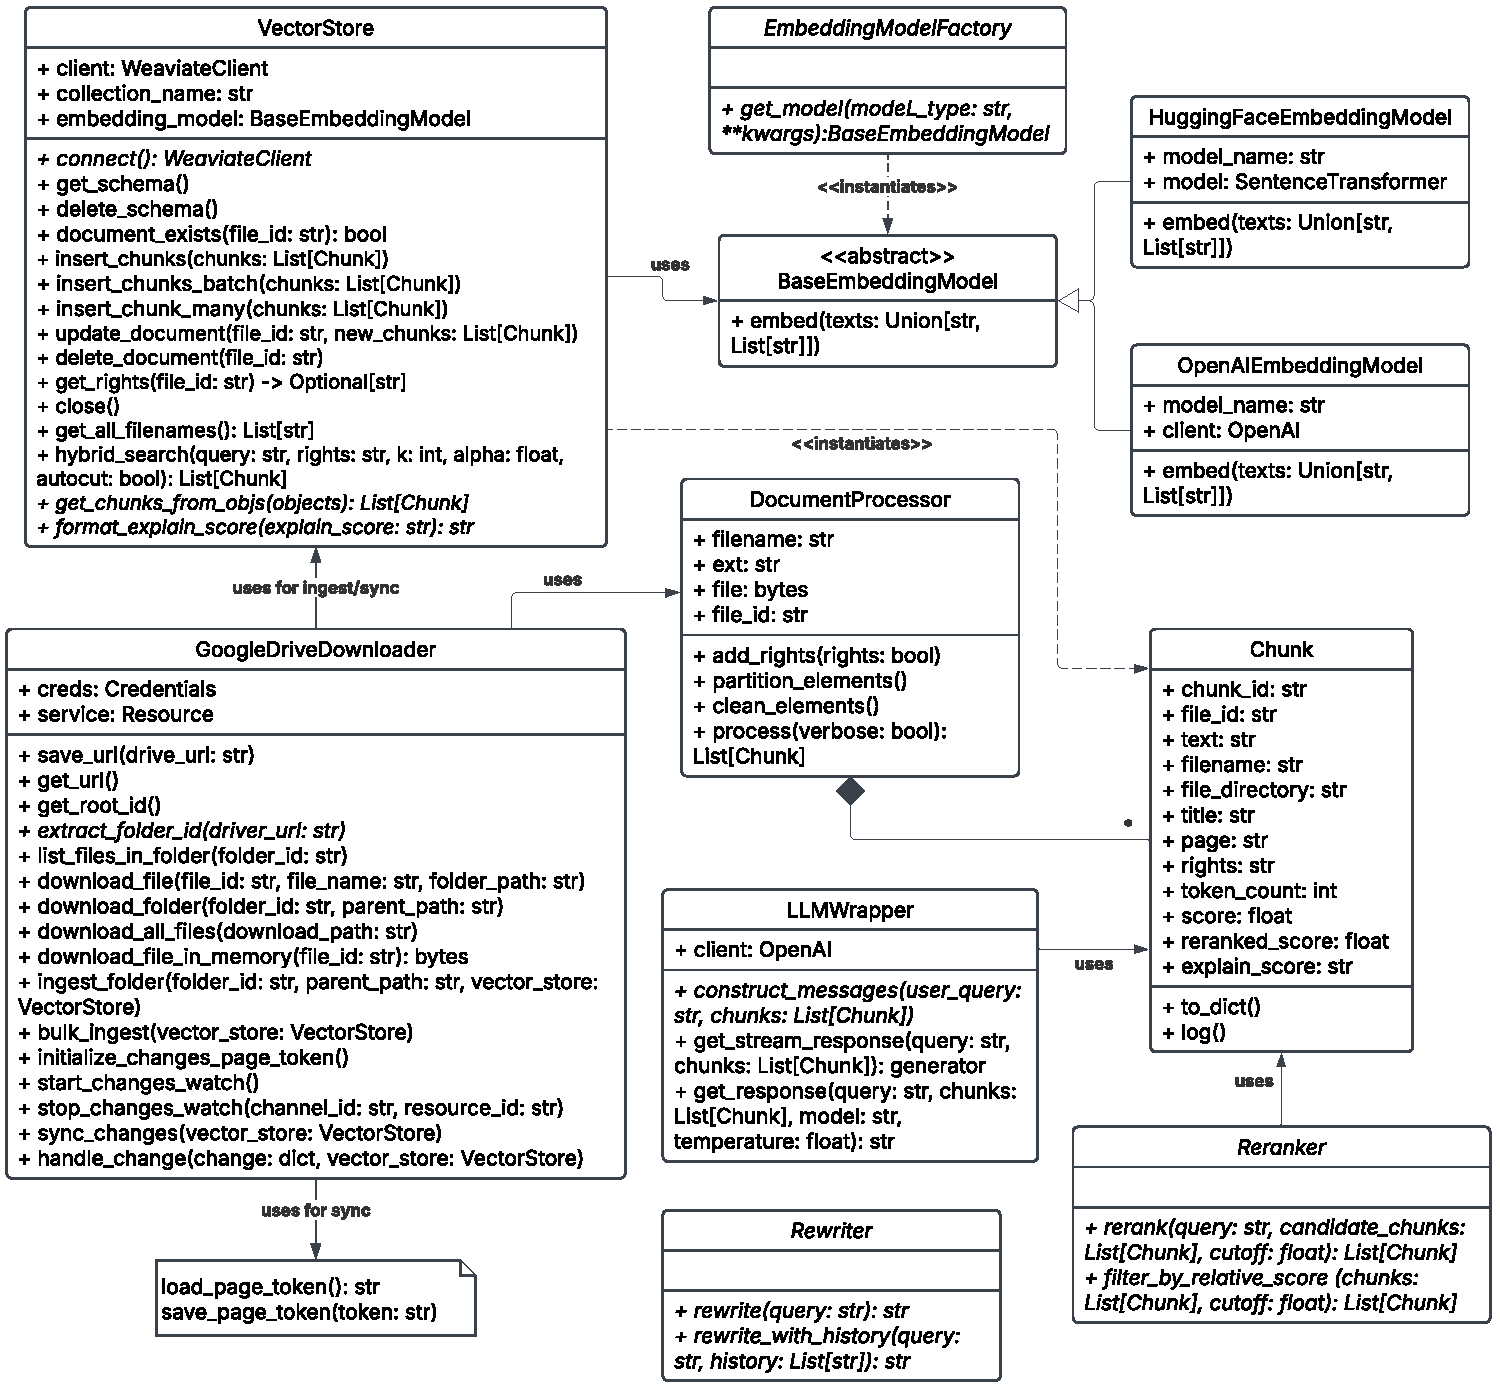
\includegraphics[width=1\linewidth]{obrazky/RAG class diagram.pdf}
    \caption{Diagram tříd. Kurzívou jsou označneny statické metody.}
    \label{fig:class}
\end{figure}

\subsection{\texttt{DocumentProcessor}}
Třída \texttt{DocumentProcessor} slouží ke zpracování dokumentů. Při inicializaci obdrží cestu k lokálně uloženému dokumentu nebo dokument v paměti po bytech. Metoda \texttt{process()} pak vrací seznam vytvořených chunků k uložení do databáze. Zpracování probíhá ve třech krocích:
\begin{enumerate}
    \item \textbf{Extrakce textu} je realizována pomocí knihovny \texttt{Unstructured}~\cite{unstructured}. Ta poskytuje metody \texttt{partition()} pro různé typy souborů, které mají všechny výstupem seznam elementů reprezentujících logické celky dokumentu. Každý element obsahuje extrahovaný text, metadata a kategorii popisující účel v dokumentu (např. záhlaví, narativní text, nadpis apod. – možné kategorie elementu se odvíjí od typu dokumentu). \texttt{Unstructured} je high-level knihovna a pro zpracování různých typů souborů využívá externí nástroje, které je třeba mít nainstalované:
    \begin{itemize}
        \item pro \texttt{.doc} a \texttt{.docx} je zapotřebí \texttt{libreoffice},
        \item pro binární soubory jako \texttt{.pdf}, \texttt{.jpg}, \texttt{.png} a \texttt{.heic} slouží k extrakci textu optické rozpoznávání znaků (OCR) za použití modulu \texttt{tesseract},
        \item nástroj \texttt{poppler} je pak využíván k renderování \texttt{.pdf} dokumentů.
    \end{itemize}
    \item \textbf{Čištění textu} je mezikrokem zpracování a upravuje podobu textu pro lepší výsledky chunkování především odstraněním přebytečných mezer, emoji a odrážek v seznamech. Konfigurovatelným krokem k předpovídatelné struktuře datasetu je pak detekce nezaznamenaných nebo naopak odstranění přebytečných nadpisů, což vede k lepšímu dělení textu.
    \item \textbf{Chunkování} je implementováno podle principu popsaného v kapitole~\ref{chunking}. 
    
    Text jednotlivých elementů je dělen na věty. Věty jsou detekovány pomocí funkce \texttt{nltk.tokenize.sent\_tokenize(text)}~\cite{nltk} a dále analyzovány na počet tokenů. O tokenizaci se stará \texttt{AutoTokenizer}~\cite{tokenizerhuggingface}, jehož architektura je odvozena od použitého embedding modelu.
    
    Embedding model \texttt{all-mpnet-base-v2}, pro který jsou chunky připravovány, má limit 384 tokenů na vstupu a tomu je velikost chunku přizpůsobena, jelikož přesah limitu vstupu tento embedding model zahazuje. Menší chunky by naopak nemusely poskytnout dostatek kontextu.

    Pro uzavření chunku a vytvoření nového slouží mimo limit taky detekce nadpisů. Ta využívá kategorii elementů \texttt{Title}.
\end{enumerate}

\subsection{\texttt{EmbeddingModel}}
Pro výběr embedding modelu byla navržena abstraktní třída \texttt{BaseEmbeddingModel} definující rozhraní \texttt{embed()}. Ta slouží jako základ pro komponentu embedding modelu, která je zodpovědná za vektorizaci textových pasáží chunků pro uložení do vektorové databáze a také vektorizaci dotazu pro následné vyhledávání.

Třída \texttt{HuggingFaceEmbeddingModel} využívá modely ze sady \texttt{sentence-transformers}. Pro systém byl využit model \texttt{all-mpnet-base-v2}, který je navržen pro obecné použití a z dostupných modelů poskytuje nejlepší kvalitu, je však pomalejší oproti běžně používanému \texttt{all-MiniLM-L6-v2}~\cite{sentence-tranformers}.  

Třída \texttt{OpenAIEmbeddingModel} využívá rozhraní OpenAI API k získání embeddingů~\cite{openaidocs}. Tento způsob byl zkoumán jako alternativní, nicméně tato služba je zploplatněná, a tak bylo preferováno využití lokálního modelu pro finální verzi systému. 

Výběr konkrétní implementace se provádí tovární třídou \texttt{EmbeddingModelFactory}, která podle parametru \texttt{model\_type} vrací odpovídající instanci embedding modelu.

\subsection{\texttt{VectorStore}}
Pro implementaci externího úložiště znalostí s hybridním vyhledáváním byla využita open-source vektorová databáze Weaviate~\cite{weaviate}, která poskytuje jednoduché řešení pro vývoj v docker kontejneru podporující hybridní vyhledávání. Při každém přístupu do databáze je inicializován klient, který se k ní připojí. Pro účely ukládání chunků pak slouží jedna kolekce:
\begin{verbatim}
collection = client.collections.create(
    name=collection_name,
    vector_index_config=Configure.VectorIndex.hnsw(
        distance_metric=VectorDistances.COSINE,
    ),
    properties=[
        Property(name="chunk_id", data_type=DataType.TEXT),
        Property(name="file_id", data_type=DataType.TEXT),
        Property(name="text", data_type=DataType.TEXT),
        Property(name="filename", data_type=DataType.TEXT),
        Property(name="file_directory", data_type=DataType.TEXT),
        Property(name="title", data_type=DataType.TEXT),
        Property(name="page", data_type=DataType.TEXT),
        Property(name="rights", data_type=DataType.TEXT)
    ],
)
\end{verbatim}
Konfigurace kolekce využívá HNSW (viz~\ref{grafove metody}) k indexaci a kosinovu podobnost jako podobností funkci při vektorovém vyhledávání, které je kombinováno s BM25 do hybridního vyhledávání. Strategie vyhledávání byla zvolena na základě testování a evaluace systému (kap. \ref{evaluace}) následovně:
\begin{verbatim}
response = collection.query.hybrid(
    query=query,
    vector=embedding_model.embed(query)[0],
    alpha=0.55,
    fusion_type=HybridFusion.RELATIVE_SCORE,
    return_metadata=MetadataQuery(score=True, explain_score=True),
    auto_limit=3,
    filters=Filter.by_property("rights").equal(rights)
)
\end{verbatim}
\texttt{HybridFusion.RELATIVE\_SCORE} označuje algoritmus sloučení hybridního skóre, kde relativní skóre je vyjádřeno vzorcem zmíněným v kapitole~\ref{hybrid}. Parametr \texttt{auto-limit} představuje tzv. \textit{autocut}, který nevrací pevný počet vyhledaných záznamů, ale $k$ prvních shluků záznamů dle skóre. Tento přístup tak dokáže navracet variabilní počet nejrelevantnějších chunků. Jelikož dotazy mohou být vágní a nemířit tak na konkrétní informace, je tento parametr nastaven volněji, aby byl vyhledán širší kontext relevantních chunků, jenž je zpracován rerankingem. Dále je aplikován filtr dle přístupových práv uživatele k ilustraci metadata filtrování.

\subsection{\texttt{Rewriter}}
\label{rewriter}
Modul \texttt{Rewriter} zaobaluje oba jeho módy. Statická metoda \texttt{rewrite()} využívá OpenAI API~\cite{openaidocs} pro volání modelu \texttt{gpt-4o} k přeformulování dotazu uživatele do podoby optimalizovanější pro vyhledávání. Použitý prompt vypadá následovně:
\begin{verbatim}
system:   You are a query rewriting assistant in a Retrieval-Augmented 
Generation (RAG) system that uses both semantic and keyword-based search 
(hybrid retrieval).

Your task is to rewrite user queries to improve retrieval performance by:
- Making the query **more specific, structured, and searchable**.
- Emphasizing **important keywords or phrases** that are likely to appear 
  in source documents.
- Removing filler phrases like 'tell me about', 'please explain', 'can you
  describe', etc.
- Avoiding full-sentence questions unless absolutely necessary.
- Keeping the rewritten query as **concise and retrieval-friendly** 
as possible.
- Never adding assumptions or new topics not present in the original query.
- If the query is nonsensical, return it unchanged.

Examples:
- Input: 'Tell me something about AI agents' → Output: 'AI agents overview'
- Input: 'Can you explain vector databases in machine learning?' → Output: 
  'vector databases in machine learning'
- Input: 'aodwhuoaed' → Output: 'aodwhuoaed'

user:   {query}
\end{verbatim}

Podporu chatové historie a navazujících dotazů řeší metoda \texttt{rewrite\_with\_history()}, lišící se promptem, který zahrnuje i poslední 3 páry dotaz–odpověď pro uvedení kontextu pro přeformulání dotazu, pakliže je neúplný:

\begin{verbatim}
system:   You are a query rewriting assistant in a Retrieval-Augmented 
Generation (RAG) system that uses both semantic and keyword-based search
(hybrid retrieval).
    
Your task is to rewrite user queries to improve retrieval performance by:
- Keep the rewritten query semantically equivalent to the original while 
  keeping the keywords.
- Do NOT add information or assumptions not present in the original query
  or context.
- If the query is nonsensical, too short, or unrewritable, just return it
  unchanged.

The user query may be a follow-up question. Use the recent chat history
below **only to resolve ambiguous or incomplete queries**. 
Recent Chat History:

Q: {history_question}
A: {history_answer}

...

user:   {query}
\end{verbatim}

\subsection{\texttt{Reranker}}
\label{reranker}
Modul \texttt{Reranker} mění pořadí a upřesňuje míru relevance chunků, které byly vyhledány. Využívá model \texttt{cross-encoder/ms-marco-MiniLM-L-6-v2}~\cite{crossencoder}. Pomocí metody \texttt{rank(query, candidates)} pak určuje skóre relevance, dle kterého jsou chunky nově řazeny pro formulaci kontextu. Skóre se pohybuje přibližně v intervalu $[-10, 10]$.

Na nově seřazené chunky je aplikován filtr pomocí metody \texttt{filter\_by\_relative\_score (chunks, cutoff)}. Ta nejprve posune všechna skóre rerankingu do kladných hodnot, aby následně mohla vypočíst práh jako podíl z maximálního skóre danou parametrem \texttt{cutoff}, jehož hodnota byla evaluací (kap.~\ref{cutoff}) stanovena na \textbf{0.5}. Tento výpočet bere v úvahu dynamickou podobu rozsahu skóre rerankingu jednotlivých záznamů. Vyhledané záznamy se skórem nižším než tento vypočtený práh jsou označeny za nerelevantní vyřazením z kontextu.

\subsection{\texttt{LLMWrapper}}
\label{llmwrapper}
Nadstavbu nad voláním jazykového modelu obstarává modul \texttt{LLMWrapper}. Vstupem je dotaz a chunky tvořící kontext k zodpovězení dotazu. Prvním krokem je sestavení promptu, který definuje instrukce pro model a formát očekávané odpovědi:

\begin{verbatim}
system:   You are a factual answer generator in a Retrieval-Augmented 
Generation (RAG) system.
            
You will receive a user query and a list of context chunks retrieved from 
a document store. Each chunk contains text from a specific file, with 
optional section titles or page numbers.

Your job is to answer the user's question using **only** the provided 
context. Cite the sources used in your answer using the format: 
[File: filename, Section: title, Page: page]. If section or page is
missing, omit them from the citation.

**Rules:**
- Do NOT use any knowledge outside the context.
- Do NOT speculate or invent information.
- If at least one chunk contains relevant information, answer using only 
  that content.
- Do NOT include a fallback message unless **none** of the chunks are even
  partially relevant.
- Do NOT try to give an exhaustive answer — partial answers are acceptable.
- Do NOT explain what is missing.
- Format your answer using **markdown**, be **short and factual**, and
  avoid repetition.

If there is truly no relevant information in any chunk, respond with:
My knowledge base does not provide information for this query.



Context:
[File: {filename}, Section: {title}, Page: {page}]
{text}

...

user:   {query}
\end{verbatim}

Druhým krokem je samotné volání jazykového modelu, které probíhá prostřednictvím rozhraní OpenAI API~\cite{openaidocs} za využití modelu \texttt{gpt-4o}, přičemž odpověď je generována po částech formou \textit{streamu}, čímž se zlepšuje vnímání odezvy systému ze strany uživatele. Teplota modelu je nastavena na nízkou hodnotu $0.2$, což zajišťuje konzistentnější odpověď a nižší míru kreativity odpovědi, vhodnou pro Q\&A.

Kód pro generování odpovědi pak vypádá následovně:
\begin{verbatim}
stream = client.chat.completions.create(
    model="gpt-4o",
    messages=prompt,
    temperature=0.2
    stream=True
)

for response in stream:
    yield response.choices[0].delta.content
\end{verbatim}

\subsection{\texttt{GoogleDriveDownloader}}

Třída \texttt{GoogleDriveDownloader} zajišťuje integraci systému s cloudovým úložištěm Google Drive. Jejím úkolem je stažení a synchronizace dokumentů tvořících znalostní bázi, a to jak v rámci prvotního zpracování, tak průběžně pomocí sledování změn.

Dokumenty jsou z cloudu stahovány metodou \texttt{download\_file\_in\_memory()}, která vrací binární obsah dokumentu, který je předán ke zpracování a nahrán do databáze. Tento proces tak probíhá přímo v paměti bez nutnosti uložení na disk. 

Při připojení složky je provedeno prvotní nahrání všech dokumentů realizováno v rámci metody \texttt{bulk\_ingest()}. Dokumenty složky jsou zpracovávány rekurzivně včetně vnořených podadresářů.

Pro zajištění automatické synchronizace stavu dokumentů využívá třída API rozhraní \texttt{Google Drive Changes API}~\cite{googledriveapi}. Metodou \texttt{start\_changes\_watch()} je registrován tzv. \textit{webhook}, který upozorňuje systém na každou změnu. Tyto změny jsou zpracovány metodou \texttt{sync\_changes()}, která využívá \texttt{page\_token}, který identifikuje poslední stav změn. To umožňuje získat pouze změny od poslední synchronizace, které jsou obstarávány metodou \texttt{handle\_change()} pro učinění změn (nový dokument, aktualizace, smazání).

\newpage

\section{API}
Serverová část systému komunikuje s frontendem skrze API realizované webovým frameworkem FastAPI. 

\subsection{API endpointy}
\begin{itemize}
    \item \texttt{/driveurl} – Ukládá URL sledované složky.
    \item \texttt{/ingest\_folder} – Provádí prvotní nahrání dokumentů složky do vektorové databáze metodou \texttt{bulk\_ingest()} třídy \texttt{GoogleDriveDownloader}.
    \item \texttt{/delete\_schema} – Smaže celou databázi.
    \item \texttt{/query} – Provádí celý proces vyhledávání a vrácí odpověď v podobě \textit{streamu}.
    \item \texttt{/webhook} – Obstarává přicházející notifikace změn ve sledované složce cloudového úložiště Google Drive.
    \item \texttt{/sync} – Manuálně spouští synchornizaci změn  sledované složky.
    \item \texttt{/filenames} – Vypíše názvy dokumentů uložených v databázi.
\end{itemize}

\subsection{Webhook}
Koncový bod \texttt{/webhook} je pro \texttt{Google Drive Changes API} \cite{googledriveapi} zvěřejněn pomocí nástroje \texttt{ngrok}~\cite{ngrok}. Tím je zajištěno, že při jakýchkoliv změnách provedených ve sledované složce bude odeslána zpráva na tento koncový bod. Ten pak přijímá parametr \texttt{resource\_state}, který označuje stav příchozí zprávy. Při stavu \texttt{changes} je zapnuta synchronizační rutina.

\subsection{StreamingResponse}
Koncový bod API \texttt{/query} vrací \texttt{StreamingResponse}~\cite{fastapi} pro poskytnutí odpovědi po částech tak, jak je generována. Na frontend posílá tok zpráv ve formátu JSON, přičemž první zpráva obsahuje serializované chunky, které byly použity pro tvorbu kontextu, a zbytek zpráv tvoří odpověď z generátoru, který vrací \texttt{LLMWrapper}. Generátor, sloužící jako vstup pro \texttt{StreamingResponse}, pak vypadá následovně:
\begin{verbatim}
def stream():
    serialized_chunks = [vars(chunk) for chunk in reranked_chunks]
    yield json.dumps({
        "text": None,
        "metadata": {"chunks": serialized_chunks}
    }) + "\n"
    for llm_response in llm_wrapper.get_stream_response(
        query, reranked_chunks
    ):
        response.append(llm_response)
        yield json.dumps({
            "text": llm_response,
            "metadata": None
        }) + "\n"

\end{verbatim}

\section{Uživatelské rozhraní}

Uživatelské rozhraní slouží jako hlavní přístupový bod pro uživatele systému. Je navrženo jako webová aplikace s cílem umožnit pohodlné dotazování nad vlastní znalostní bází. 

Webové rozhraní je vytvořeno pomocí frameworku Vue.js, nastylovaná utility-first frameworkem Tailwind CSS a komunikace s backendem probíhá prostřednictvím REST API. Aplikace podporuje streamování odpovědi od jazykového modelu po jednotlivých blocích, což zlepšuje uživatelský dojem a snižuje vnímanou dobu odezvy. 

Pro demonstraci funkcionality jsou k dispozici 2 pohledy. Uživatelský pohled zobrazuje zamýšlené rozhraní s dotazy a odpovědmi, zatímco vývojářský pohled zobrazuje k daným dotazům vyhledané chunky a jejich skóre, které tvořily kontext pro odpověď. Dále je možné vypnout nebo zapnout chatovou historii a přepínat role uživatele pro filtrování dle přístupových práv.

\begin{figure}[H]
    \centering
    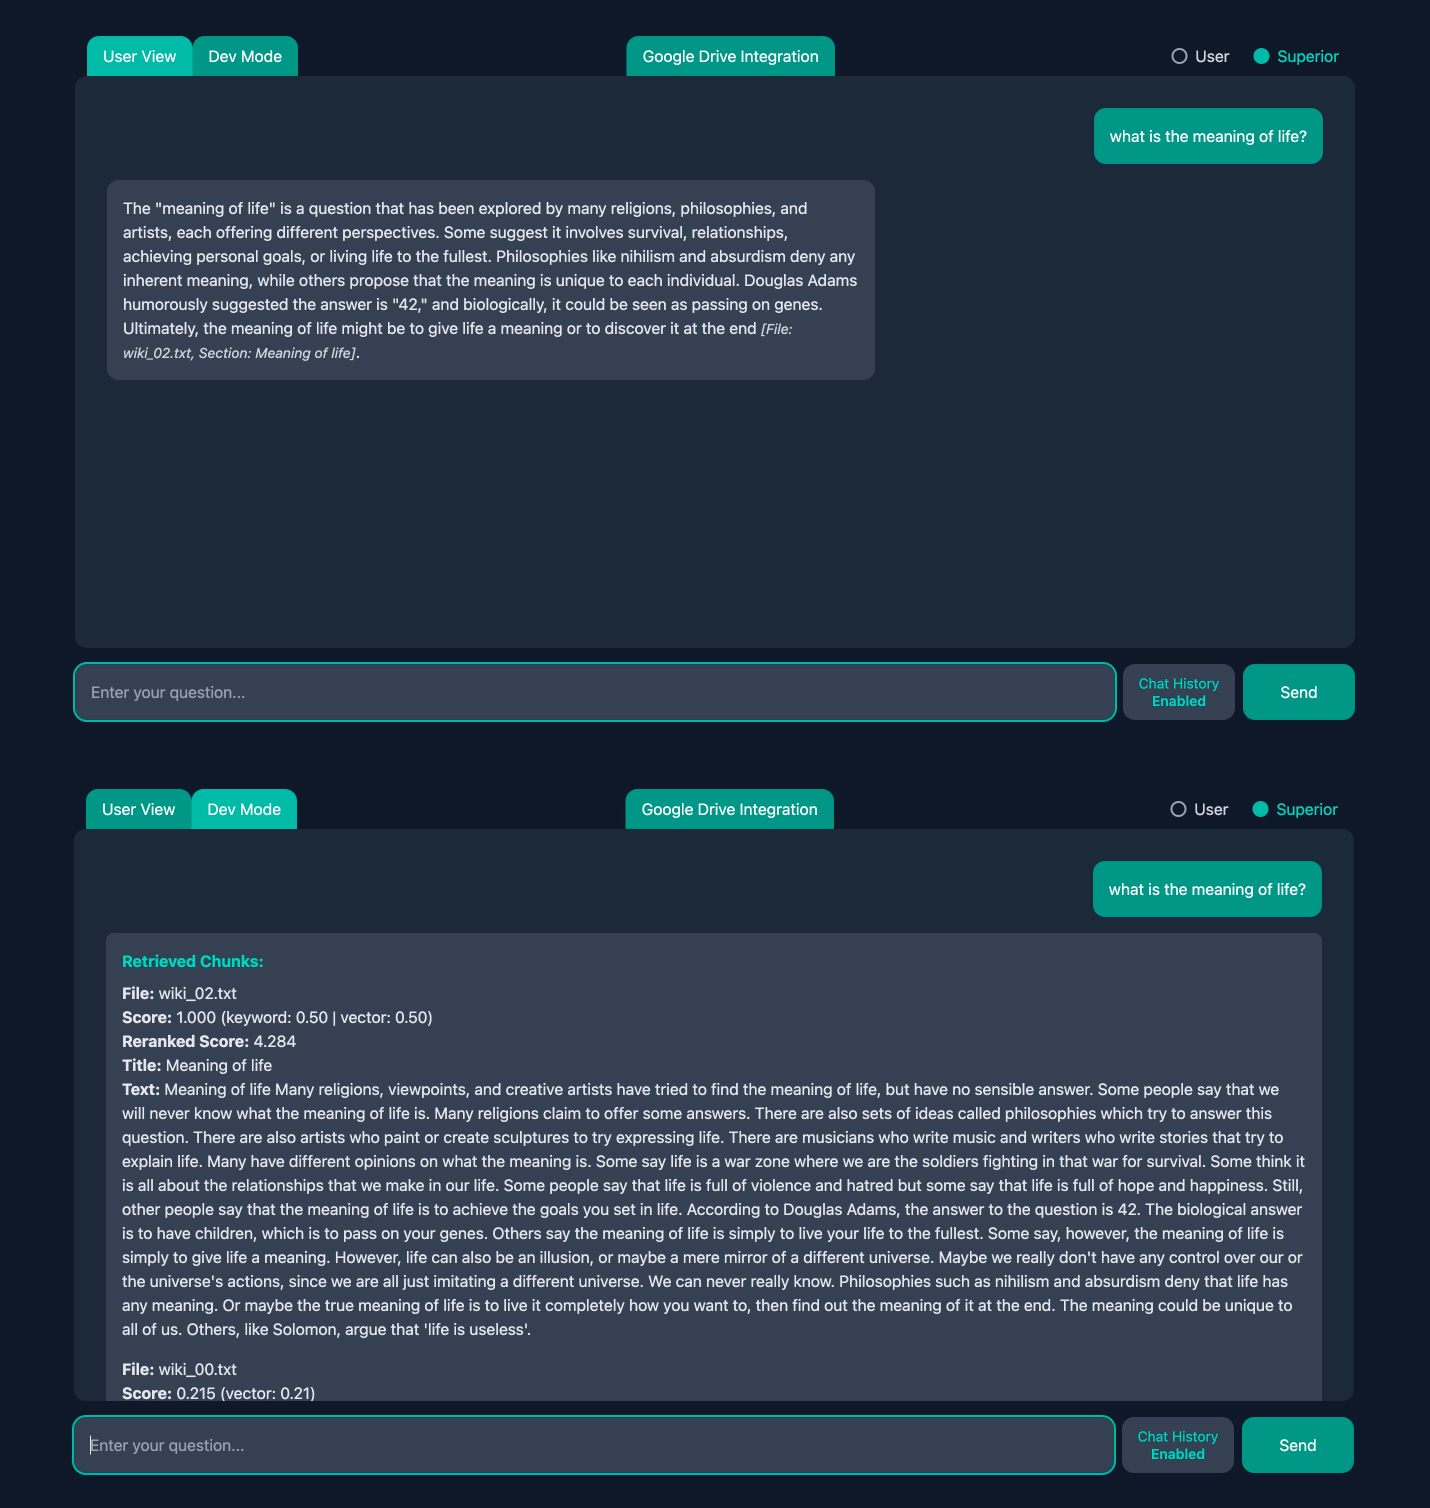
\includegraphics[width=0.97\linewidth]{obrazky/ui.png}
    \caption{Webová aplikace: nahoře je pohled uživatele a dole je pohled vývojáře}
    \label{fig:gui}
\end{figure}



\chapter{Testování a evaluace}
\label{evaluace}
% testování
% dataset, kritéria hodnocení, výsledky
% Kontext a návaznost na předchozí kapitolu o evaluaci RAG
% Důvody a cíle testování
% Přehled hlavních evaluačních přístupů (retrieval, RAGAs)
% Struktura kapitoly
% LLM as judge 

V kapitole~\ref{evaluaceteorie} byla diskutována teoretická východiska evaluace RAG systémů, která poukazují na komplexnost samotného hodnocení. Cílem této kapitoly je experimentálně ověřit výkonnost implementovaného systému na konkrétním datovém vzorku s využitím zvolených evaluačních metod.

Nejprve je popsán použitý dataset a jeho rozdělení pro jednotlivé typy testování. Evaluace poté probíhá na dvou úrovních: 
\begin{enumerate}
    \item Testování vyhledávacího modulu, kde je ověřena schopnost systému vyhledávat dokumenty, přesněji jejich relevantní části, na základě dotazu.
    \item Komplexní evaluace celé RAG pipeline pomocí frameworku RAGAs.
\end{enumerate}

Při tvorbě testovacích sad byl použit LLM, aby nedošlo k ovlinění lidským faktorem. Tento přístup je časově efektivní a zároveň snižuje riziko neúmyslného zkreslení, které by mohlo vzniknout při ruční formulaci dotazů. 

Výsledky přesto nelze považovat za absolutní, jelikož mimo kvalitu systému závisí výsledky na datech, na kterých je systém testován, a také na samotných dotazech. Jejich smyslem je tak poskytnout indikativní pohled na chování systému v realistickém scénáři.

\section{Dataset}
% kaggle simple english wiki dump
% popis datasetu, zdroj
% rozdělení datasetu pro jednotlivé testy (rozsah)
Pro účely testování a evaluace byl využit dataset \textit{Plain text Wikipedia (SimpleEnglish)} \footnote{https://www.kaggle.com/datasets/ffatty/plain-text-wikipedia-simpleenglish}. Jedná se o neanotovaný (nesupervidovaný) textový korpus obsahující všechny články ze Simple English Wikipedie, varianty Wikipedie psané ve zjednodušené angličtině. Extrahované články jsou předzpracovány na čistý text zbavený formátování, odkazů, šablon a jiných prvků a tvoří tak předpovídatelný formát.

Rozsah celého datasetu činí 249\,396 článků rozdělených do 171 souborů o velikosti do 1MB. Tento dataset byl zvolen především díky obsahové rozmanitosti témat, jazykové jednoduchosti a také uniformní povaze dat usnadňující zpracování. To vytváří konzistentní datovou bázi pro testování a evaluaci.

Pro testování a evaluaci byla použita podmnožina tohoto datasetu činící 30 dokumentů s články (po zpracování cca 29\,500 chunků).

% \begin{itemize}
%     \item \textbf{Retrieval testy:} 30 dokumentů (29\,500 chunků) použitých jako znalostní báze pro testování vyhledávací komponenty na základě dotazů pocházejících z konkrétních chunků,
%     \item \textbf{RAGAs evaluace:} 30 dokumentů (29\,500 chunků) s dotazy, referenčním kontextem i referenčními odpověďmi pro end-to-end evaluaci systému,
%     \item \textbf{Výkonnostní testy:} celý dataset (171 dokumentů, xxxx chunků), použitý pro měření latence a testování škálovatelnosti systému.
% \end{itemize}


\section{Testování modulu vyhledávání}
% cíl, popis testu, popis přípravy testcasů, výsledky (pro různé případy), interpretace a zhodnocení

% generated queries via ChatGPT on specific chunk to find
% matched ground truth (chunk ID)
% k-values you tested - recall@1, recall@context
% results with tables or plots.
% Insights on failure cases (e.g. context split across chunks).
Cílem této části je otestovat účinnost vyhledávacího modulu systému na schopnosti vrátit chunk obsahující odpověď na daný dotaz.

Pro každý testovací případ bylo zvoleno ID chunku ze zpracovaného datasetu a z jeho textu byl odvozen dotaz. Tyto dotazy byly generovány pomocí chatbota ChatGPT, který využíval jazykový model GPT-4-turbo a byl instruován, aby vygeneroval dotaz, který směřuje k nějaké informaci v textu sémanticky nebo pomocí klíčových slov tak, aby se odpověď na dotaz nacházela v daném chunku. Testovací soubor formátu \textit{JSON Lines} tak obsahuje 100 párů \texttt{\{query, expected\_chunk\_id\}}.

Testování probíhá formou vyhodnocení úspěšnosti retrievalu při výskytu chunku na první pozici jako nejrelevantnější chunk (Recall@1) a výskytu ve finálním kontextu (Recall@k). Jelikož jsou dotazy mířeny na konkrétní záznamy, výchozí metoda tvoření kontextu je nastavena na první shluk chunků s nejvyšším skóre (\texttt{top-k = 1, autocut}).

\subsection{Parametr $\alpha$}
Poměr mezi váhami vektorového a fulltextového vyhledávání v hybridním přístupu řídí parametr $\alpha$. V grafu~\ref{fig:alpha-recall} jsou zobrazeny výsledky testu pro celý rozsah parametru k vyhodnocení: $\alpha \in \langle 0, 1 \rangle$ po krocích $0.05$.

Nejlepších hodnot metrik Recall@1 a Recall@k bylo dosaženo při $\alpha = 0{,}55$, což odpovídá vyváženému poměru mezi oběma typy vyhledávání mírně inklinujícímu k vektorovému, které se projevilo v testování jako silnější. Výrazné omezení jednoho z přístupů k vyhledávání však vede ke zhoršení výkonu, což potvrzuje předpokladáný výsledek a smysl použití hybridního vyhledávání.

\begin{figure}[H]
    \centering
    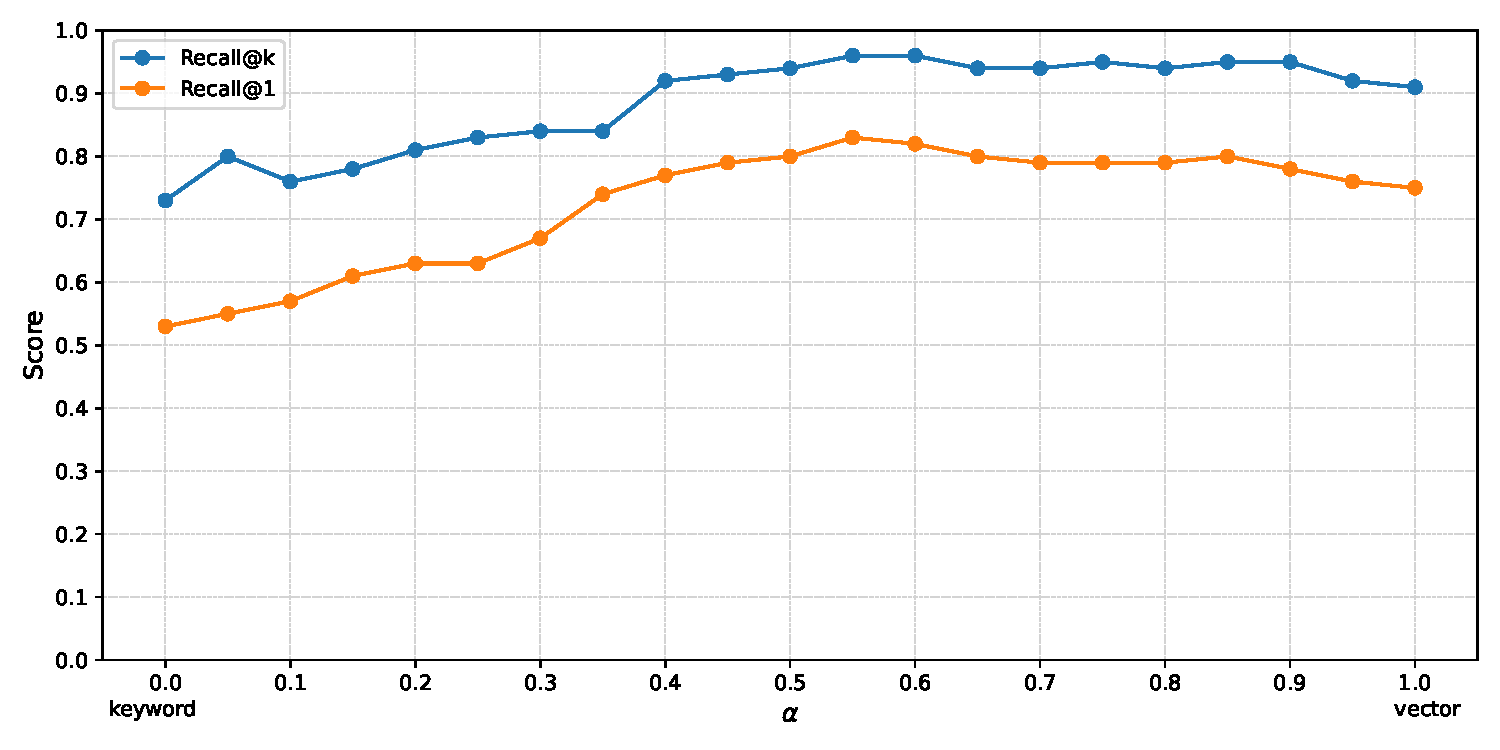
\includegraphics[width=\linewidth]{obrazky/alpha_recall.pdf}
    \caption{Porovnání Recall@1 a Recall@k pro různé hodnoty parametru $\alpha$ při hybridním vyhledávání bez rerankingu, kde kontext tvoří první shluk chunků }
    \label{fig:alpha-recall}
\end{figure}

\subsection{Strategie vyhledávání a vliv rerankingu}
Reranking má vliv nejen na pořadí chunků ve výsledku, ale také na výslednou velikost kontextu, který je následně předáván jazykovému modelu. To ilustrují výsledky v tabulce~\ref{tab:retrieval_metrics_full}. Test probíhal hybridním vyhledáváním ($\alpha=0.55$) se zapnutým/vypnutým rerankingem pro hodnoty \texttt{top-k} $\in \{1,\  2,\ 3\}$ pro prozkoumání širšího kontextu a při rerankingu také pro hodnoty \texttt{cutoff} $\in \{0.3,\ 0.5,\ 0.7\}$ filtračního prahu (parametr filtrační funkce modulu \texttt{Reranker} – kap.~\ref{reranker}). 

\begin{table}[H]
    \centering
    \label{tab:retrieval_metrics_full}
    \renewcommand{\arraystretch}{1.2}
    \begin{tabular}{|c|c|c|c|c|c|}
        \hline
        \textbf{top-k} & \textbf{cutoff} & \textbf{Recall@1} & \textbf{Recall@k} & \textbf{Rank} & \textbf{Context size} \\
        \hline
        \multirow{4}{*}{1} 
        & off   & 0.83 & 0.96 & 1.18 & 2.57 \\
        & 0.3   & 0.86 & 0.93 & 1.08 & 1.53 \\
        & 0.5   & 0.86 & 0.93 & 1.08 & 1.38 \\
        & 0.7   & 0.86 & 0.91 & 1.05 & 1.23 \\
        \hline
        \multirow{4}{*}{2} 
        & off   & 0.83 & 0.97 & 1.21 & 8.80 \\
        & 0.3   & 0.84 & 0.96 & 1.15 & 3.86 \\
        & 0.5   & 0.84 & 0.96 & 1.15 & 2.45 \\
        & 0.7   & 0.84 & 0.95 & 1.13 & 1.59 \\
        \hline
        \multirow{4}{*}{3} 
        & off   & 0.83 & 0.98 & 1.27 & 17.58 \\
        & 0.3   & 0.82 & 0.97 & 1.18 & 7.52 \\
        & 0.5   & 0.82 & 0.97 & 1.18 & 3.67 \\
        & 0.7   & 0.82 & 0.96 & 1.17 & 1.90 \\
        \hline
    \end{tabular}
    \caption{Porovnání Recall@1 a Recall@k, průměrného pořadí referenčního chunku a průměrné velikosti kontextu, hodnota \texttt{off} sloupce \texttt{cutoff} značí vypnutý reranking}
\end{table}

Výsledky ukazují, že samotné hybridní vyhledávání dosahuje dobrých výsledků, jelikož v 96\% případů byl chunk poskytující odpověď zahrnut v kontextu. Při testování se reranking neprojevil jako výrazné zlepšení výsledků. Z hodnot průměrného pořadí referenčního chunku je však patrné, že reranking dokáže přesněji odhalit sémantické detaily a většinově to tak vedlo k mírnému zlepšení Recall@1. Menší velikost kontextu pak má smysl za účelem redukce šumu, ale může také vést ke snížení nákladů na provozování systému. Vyšší míra filtrace však potenciálně vedla k horším hodnotám Recall@k. Dochází tak ke kompromisu mezi velikostí a přesností kontextu.   

\subsection{Vliv rewritingu}
Rewriting potenciálně zlepšuje vyhledávání přeformulováním dotazu, v tomto testu však při použití modulu \texttt{Rewriter} došlo ke snížení hodnot metriky Recall@1 z $0.83$ na $0.79$ a metriky Recall@k z $0.96$ na $0.93$ (při výchozí konfiguraci a parametru $\alpha=0.55$). Nepotvrdil se tedy pozitivní vliv, avšak dotazy v testovací sadě jsou již vhodně a napřímo formulované jazykovým modelem.


% \begin{table}[H]
% \centering
% \begin{tabular}{c|l|c|c|c|c}
% \textbf{TOP\_K} & \textbf{Reranking} & \textbf{Recall@1} & \textbf{Recall@k} & \textbf{Avg. rank} & \textbf{Context size} \\\hline
% \multirow{2}{*}{1} & Ne  & 0.86 & \textbf{0.96} & 1.16 & 2.34 \\
%                    & Ano & \textbf{0.89} & 0.93 & \textbf{1.05} & \textbf{1.23} \\\hline
% \multirow{2}{*}{2} & Ne  & 0.86 & \textbf{0.98} & 1.20 & 12.02 \\
%                    & Ano & \textbf{0.90} & 0.95 & \textbf{1.07} & \textbf{2.10} \\
% \end{tabular}
% \caption{Srovnání výkonu retrievalu při různých hodnotách \texttt{TOP\_K} a použití rerankingu}
% \label{tab:rerank-topk-eval}
% \end{table}


\section{RAGAs evaluace}
V této části je hodnocena výkonnost celého RAG jako end-to-end pipeline a jsou ověřeny některé strategie nastavení systému. Hodnocení bylo provedeno pomocí nástroje RAGAs~\cite{ragas}, který umožňuje automatizovanou evaluaci pomocí LLM bez nutnosti lidského hodnocení. Jako \textit{LLM-as-a-Judge} zde slouží model \texttt{gpt-4o-mini}. Pro rozšíření sledovaných metrik oproti kapitole~\ref{ragastheory} bylo též využito referenčních odpovědí.

\subsection{Hodnotící metriky}
Níže je seznam sledovaných metrik a popis, co hodnotí:
\begin{itemize}
    \item \textbf{Context Precision} – zdali jsou vyhledané informace relevantní dotazu a v kontextu se nevyskytuje zbytečný šum,
    \item \textbf{Context Recall} – jestli obsahují vyhledané záznamy informace k poskytnutí správné odpovědi a fáze retrievalu funguje, jak má,
    % \item \textbf{Noise Sensitivity} – jak moc je systém robustní a poskytuje správné odpovědi i přes šum vyskytující se v kontextu,
    \item \textbf{Response Relevancy} – na kolik je vygenerovaná odpověď relevatní k dotazu a měří tak její užitečnost,
    \item \textbf{Faithfulness} – do jaké míry je odpověď podložena vyhledaným kontextem, což kontroluje, zdali nedochází k halucinacím,
    \item \textbf{Factual Correctness (F1 score)} – jak dobře je odpověď fakticky správná porovnáním s referenční odpovědí.
\end{itemize}
Hodnoty těchto metrik se pohybují v intervalu $\langle 0, 1 \rangle$, kde vyšší hodnota znamená lepší výsledek. K těmto metrikám pak byl přidán ukazatel průměrné velikosti vstupního dotazu jazykového modelu:
% (s výjimkou \textit{Noise Sensitivity}, kde nižší hodnota znamená menší citlivost na šum a tím zaručuje lepší odolnost)
\begin{itemize}
    \item \textbf{Average input tokens} – průměrný počet tokenů v promptu, čímž je sledována velikost poskytnutého kontextu.
\end{itemize}

\subsection{Příprava testovací sady}
Modul \texttt{TestsetGenerator}, který je součástí frameworku RAGAs, využívá embedding model \texttt{all-mpnet-base-v2} a jazykový model \texttt{gpt-4o-mini} pro generování testovacích případů ve formě dvojice: dotaz a tzv. \textit{golden answer} (referenční odpověd). Pro každý testovací případ byla poskytunuta část náhodně vybraného dokumentu z datasetu. Získáné testovací případy se dělí na:
\begin{itemize}
    \item \textbf{single-hop} – dotaz je zodpověditelný na základě jediné věty nebo jednoho konkrétního úseku textu,
    \item \textbf{multi-hop} – dotaz vyžaduje zkombinování více informací z různých částí dokumentu.
\end{itemize}
Tímto způsobem bylo připraveno 50 single-hop testů a 30 multi-hop testů. Každý testovací případ byl nakonec obohacen o vyhledaný kontext a vygenerovanou odpověď, které byly získány systémem s testovanou strategií.

\subsection{Strategie vyhledávání a vliv rerankingu}
\label{cutoff}
Cílem tohoto měření (na single-hop testovacích případech) je ověřit, do jaké míry může modul \texttt{Reranker} zvýšit výkon systému při end-to-end evaluaci. Výchozí konfigurace spoléhá na hybridní vyhledávání prvního shluku zaznámů (\texttt{top-k = 1}), použití rerankingu však umožňuje nejprve načíst širší množinu relevantních informací (\texttt{top-k = 3}) a následně ji upřesnit pomocí hodnocení relevance. Testovány byly opět tři hodnoty filtračního prahu $\{0.3,\ 0.5,\ 0.7\}$. V tabulce~\ref{tab:rerank} jsou naměřené hodnoty metrik pro jednotlivé prahy.

\begin{table}[H]
\centering
\begin{tabular}{lcccc}
\toprule
\textbf{Metrika} & \textbf{Výchozí} & \multicolumn{3}{c}{\textbf{Reranker cutoff}} \\
 & & \textbf{0.3} & \textbf{0.5} & \textbf{0.7} \\
\midrule
\textbf{Context Precision}         & 0.803 & 0.837 & \textbf{0.844} & 0.833 \\
\textbf{Context Recall}            & 0.798 & 0.882 & \textbf{0.885} & 0.824 \\
\textbf{Response Relevancy}        & 0.836 & \textbf{0.890} & 0.868 & 0.832 \\
\textbf{Faithfulness}              & 0.799 & \textbf{0.885} & 0.880 & 0.777 \\
\textbf{Factual Correctness (F1)}  & 0.518 & 0.570 & \textbf{0.587} & 0.519 \\
\textbf{Avg input tokens}          & 1063  & 2585  & 1637  & 973 \\
\bottomrule
\end{tabular}
\caption{Porovnání výsledků při různých hodnotách filtračního prahu rerankingu}
\label{tab:rerank}
\end{table}

Měření ukazuje výrazný pozitivní vliv rerankingu ve všech metrikách. Zatímco hodnota prahu $0.7$ se projevila jako příliš přísná, retrieval se nejvíce zlepšil při \texttt{cutoff} $=0.5$, kde metrika Context Recall stoupnula o $0.087$. Hodnocení věrnosti a relevance odpovědi bylo nejvyšší při \texttt{cutoff} $=0.3$, avšak za cenu kontextu většího o 63\% než u hodnoty $=0.5$. 

\subsection{Velikost chunku a volba embedding modelu}
Cílem této evaluace (na single-hop testovacích případech) je zjistit optimální limit velikosti chunků a výběr embedding modelu. Jako možné scénaře byly testovány:
\begin{enumerate}
    \item \texttt{all-mpnet-base-v2}, limit 384 tokenů (limit modelu)
    \item \texttt{all-mpnet-base-v2}, limit 200 tokenů
    \item \texttt{all-MiniLM-L6-v2}, limit 256 tokenů (limit modelu)
\end{enumerate}
Oba embedding modely jsou nejlépe hodnocené z knihovny \texttt{sentence-transformers}, kde alterativní \texttt{all-MiniLM-L6-v2} vykazuje až 5x nižší latenci. Výsledky měření jsou v tabulce~\ref{tab:embedchunk}.

\begin{table}[H]
\centering
\begin{tabular}{lccc}
\toprule
\textbf{Metrika} & \textbf{1.} & \textbf{2.} & \textbf{3.} \\
\midrule
\textbf{Context Precision}         & 0.803 & \textbf{0.827} & 0.785 \\
\textbf{Context Recall}            & \textbf{0.798} & 0.686 & 0.716 \\
\textbf{Response Relevancy}        & 0.836 & \textbf{0.849} & 0.777 \\
\textbf{Faithfulness}              & \textbf{0.799} & 0.781 & 0.742 \\
\textbf{Factual Correctness (F1)}  & 0.518 & \textbf{0.571} & 0.513 \\
\textbf{Avg input tokens}          & 1063 & 801 & 772 \\
\bottomrule
\end{tabular}
\caption{Porovnání výsledků tří scénářů výběru embedding modelu a velikosti chunků (při výchozí strategii vyhledávání bez rerankingu)}
\label{tab:embedchunk}
\end{table}

Ačkoliv nabízí model \texttt{all-MiniLM-L6-v2} výrazně nižší latenci, výsledky evaluace poukazují na nižší kvalitu vyhledávání a výstupu při jeho použití. Rozdíl v limitu velikosti chunku pak nevykazuje jednoznačné výsledky pro daný dataset a testovací sadu.

\subsection{Evaluace systému}
V tab.~\ref{tab:finaleval} je evaluací ověřena úspěšnost vyhledávání a generování odpovědi pro jednodušší (single-hop) i komplexnější (multi-hop) dotazy. RAG systémy staví na vhodném nastavení parametrů a zvolení optimalizačních technik pro zlepšení výsledků, z nichž klíčové byly ověřeny v předešlém testování. Systém tak je nastaven, jak je popsáno v kapitolách~\ref{navrh} a \ref{implementace}.

\begin{table}[H]
\centering
\begin{tabular}{lcc}
\toprule
\textbf{Metrika} & \textbf{single-hop} & \textbf{multi-hop} \\
\midrule
\textbf{Context Precision}         & 0.882 & 0.678 \\
\textbf{Context Recall}            & 0.842 & 0.733 \\
\textbf{Response Relevancy}        & 0.886 & 0.778 \\
\textbf{Faithfulness}              & 0.843 & 0.848 \\
\textbf{Factual Correctness (F1)}  & 0.501 & 0.483 \\
\textbf{Avg input tokens}          & 1581 & 2156 \\
\bottomrule
\end{tabular}
\caption{Výsledky evaluace systému na single-hop a multi-hop testovacích případech}
\label{tab:finaleval}
\end{table}

Z výsledků vyplývá, že vyhledávací modul dosahuje dobrých výsledků při vyhledávání relevantních informací k přímému dotazu. Generátor pak poskytuje odpovědi relevatní dotazu a podložené informacemi z kontextu, čímž je redukován vliv halucinací. Tyto metriky mají hodnoty v rozmezí od $0{,}84$ do $0{,}89$.

F1 skóre dosahuje hodnoty pouze kolem $0{,}5$, což může naznačovat nižší faktickou správnost generovaných odpovědí. Hodnota F1 skóre vychází z porovnání generované odpovědi s předem definovanou referenční odpovědí (\textit{golden answer}). Vzhledem k tomu, že formát a rozsah odpovědi není jednoznačně definován, generátor může odpovědět správně jinou, ale stejně relevantní formulací u otevřenějších otázek. Může tak potenciálně dojít k penalizaci odpovědí, které nakonec dodávají stejně faktický obsah, jako reference.


\section{Latence}

Na výkon systému z hlediska rychlosti odezvy mají zásadní vliv především embedding model a cross-encoder. Použití rychlejšího embedding modelu (jako je \texttt{all-MiniLM-L6-v2}) a vynechání fáze rerankingu tak nabízí potenciální real-time odezvu, na úkor tomu však může klesat kvalita odpovědi. 


\chapter{Závěr}
% shrnutí výsledků, zhodnocení přínosu práce, možnosti budoucího rozvoje systému
% pdfka lip zpracovavat
% multimodal
% multilingual


%===============================================================================

% Pro kompilaci po částech (viz projekt.tex) nutno odkomentovat
%\end{document}